%step through each section of the atlas detector
%could spend more time on the muon spectrometer (like the new EE A-side detectors)
%and more time on the muon trigger
%Clare put in the minimal detail (no more than 20 pages) while Jeremy had 50 pages
%I could maybe fit somewhere in between

%need to define Muon Spectrometer (MS)
%need to define Inner Detector (ID)
%Assumptions:
%Will describe trigger


%I need to define things here like eta, pt, deltaR, etc 
%I may need to talk about isolation here
The ATLAS detector~\cite{ATLAS} is designed to measure
the products of the particle collisions produced by the LHC.
In particular, the detector seeks to measure those stable 
(or meta-stable) particles whose decay lifetime is sufficiently
long enough to interact with the detector.  This includes
a variety of fundamental particles (like muons) as well as 
composite particles (like neutrons). The wide variety of 
particles to be measured requires the implementation
of several sub-detector systems that work in tandem 
to identify and measure the properties of these particles.
The products of the LHC collisions travel in all directions, 
thus if there is any hope to measure all of the products of the collision
the detector must completely surround the collision point. 
The symmetry of the LHC dictates a cylindrically symmetric
shape for the ATLAS detector around this point.
There is another reason to build the detector to enclose
the collision point, since 
even with such a detector, the vanishingly small
cross-section of the neutrinos, which are also products
of the collision, means that these ghostly particles
will inevitably go undetected. But there is still hope!
If all other particles are measured, 
the presence of the neutrinos can be inferred 
using momentum conversation, as will be discussed later.  
In this way, the ATLAS detector is most generally suited
for measuring the wide variety of processes produced
by the LHC. 

\begin{figure}[ht!]
\centering
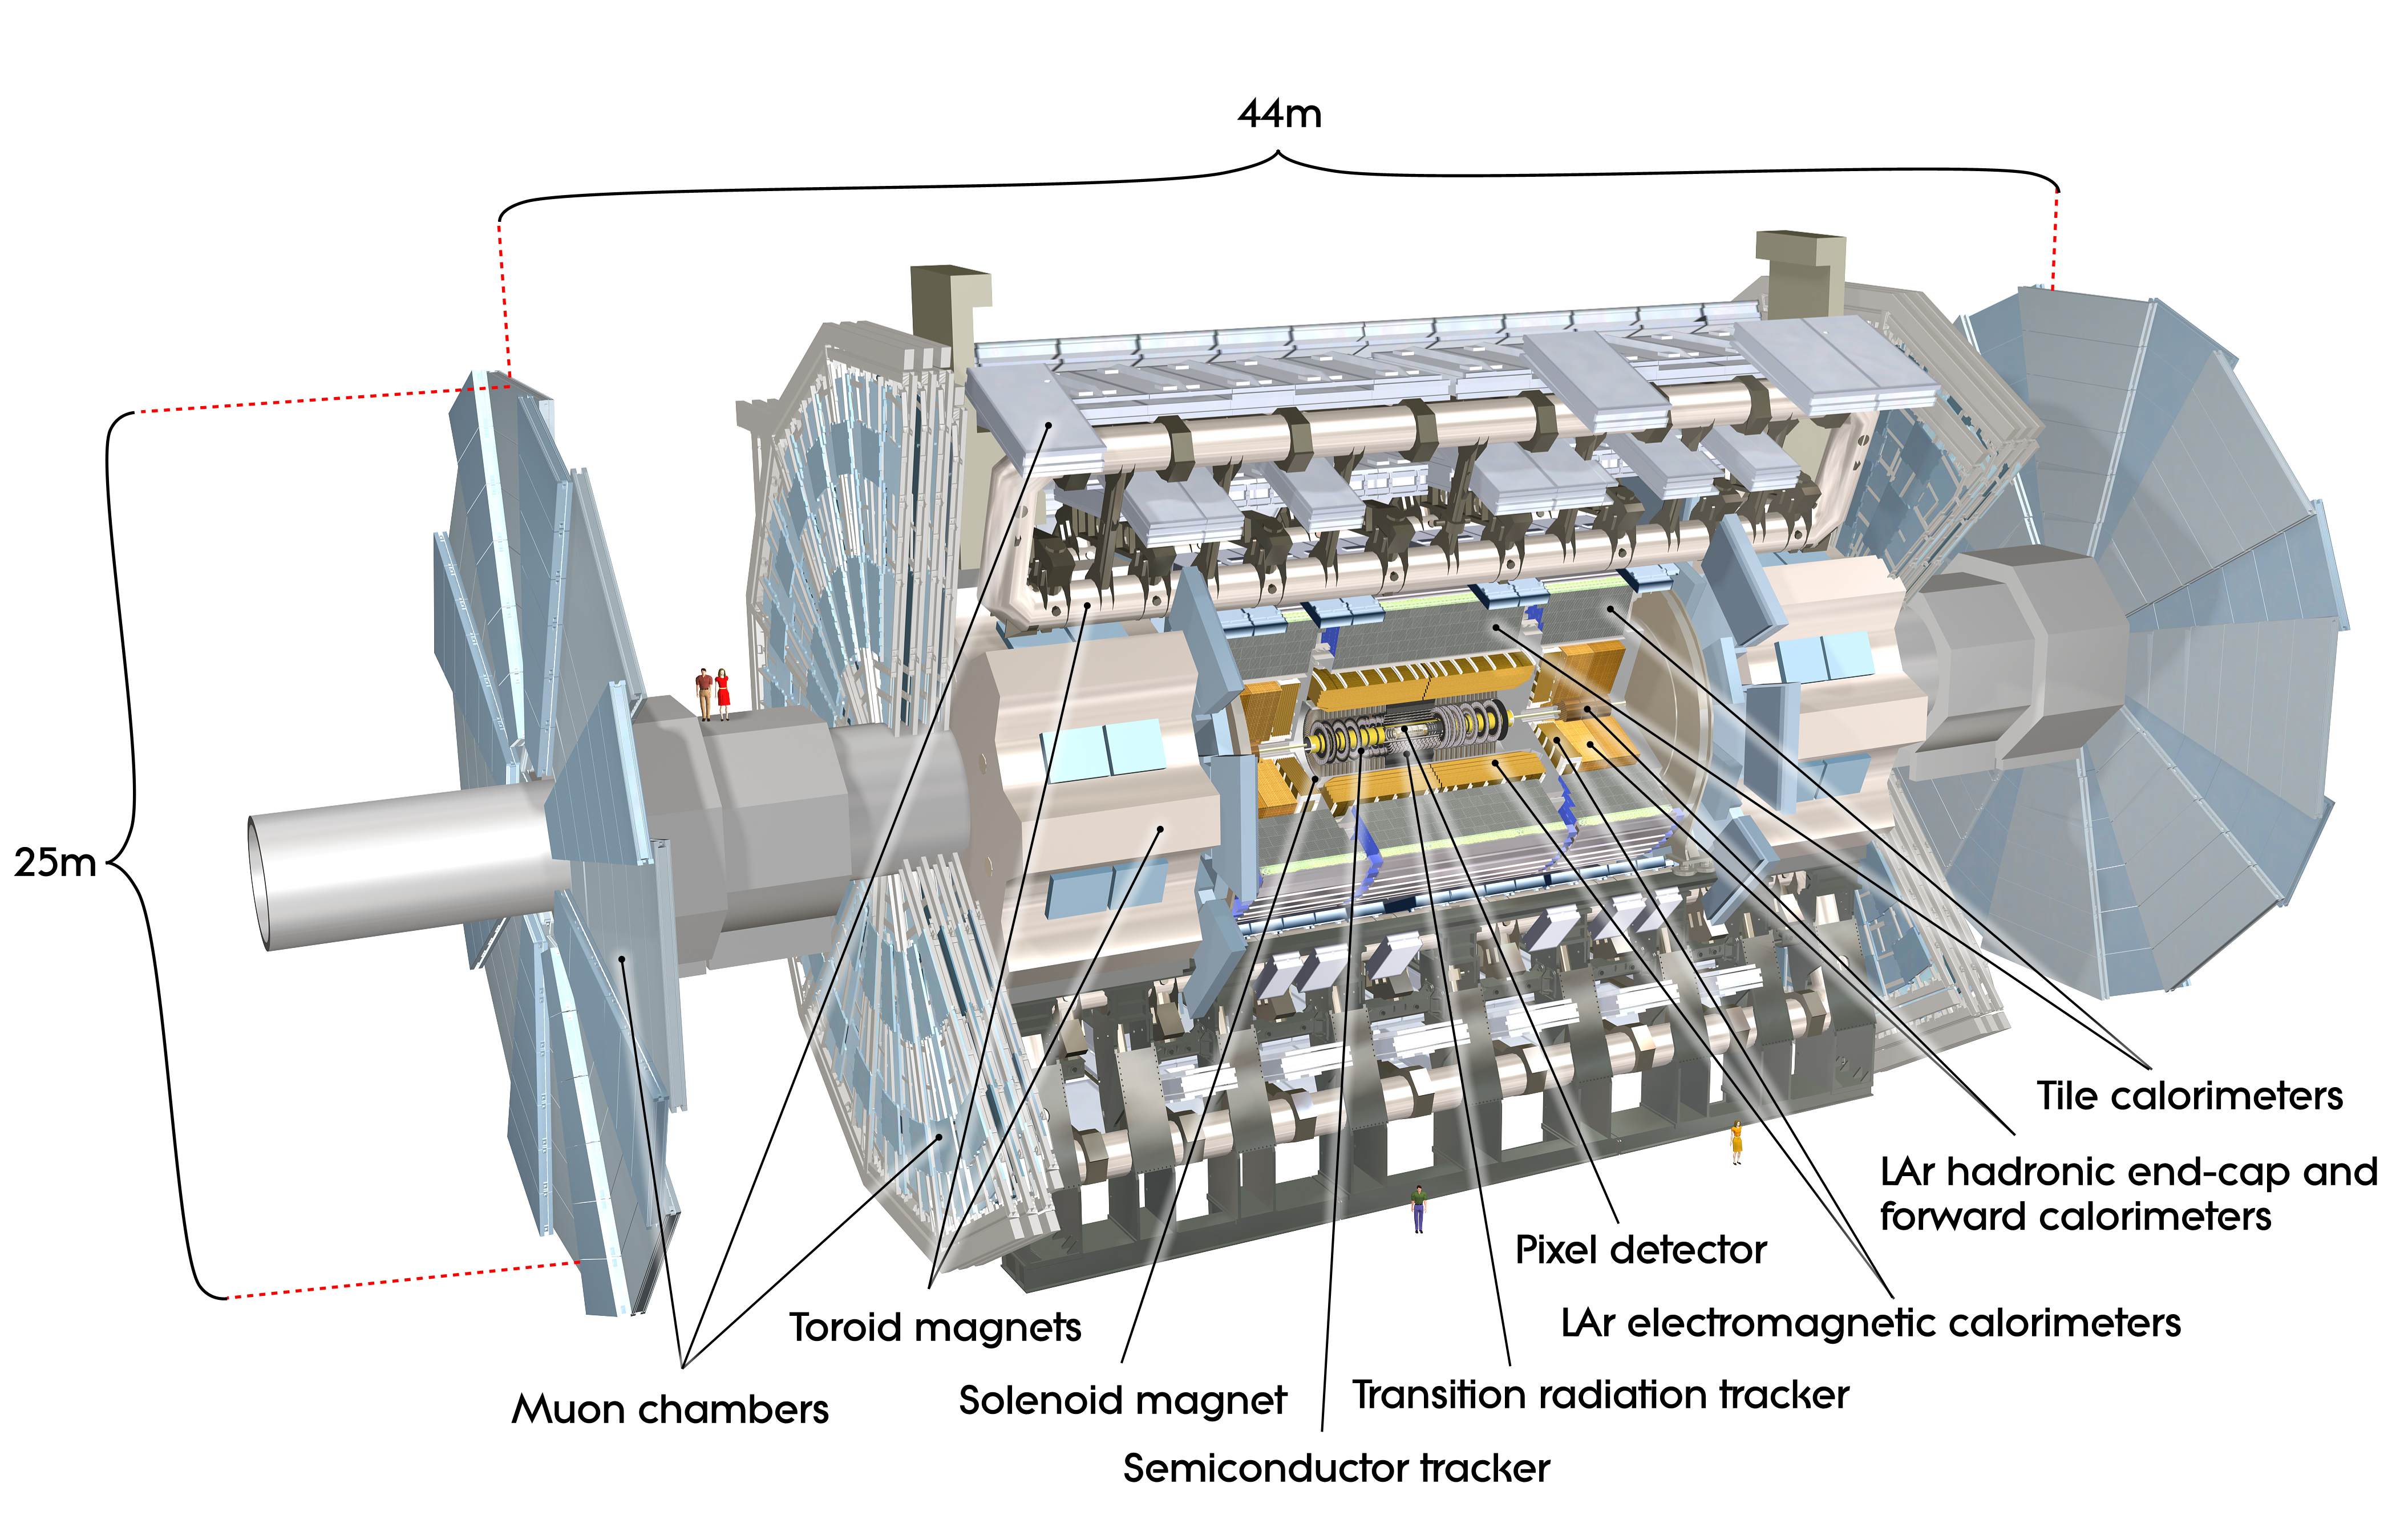
\includegraphics[width=.9\textwidth]{figures/atlas/detector.jpg}
\caption{A diagram of the ATLAS detector where the detector has
been artificially opened up to reveal the LHC beam line and the
various sub-detector components within. The sub-detector components
are labeled as such.}
\label{fig:atlas}
\end{figure}

A diagram of the ATLAS detector can be seen in \fig\ref{fig:atlas}.
It has a clearly cylindrical shape with a diameter of 25 meters
and length of 44 meters. The detector is massive, weighing
in at roughly 7000 tonnes; but it is also highly granular, with
over 100 million detection elements that are arranged very precisely, 
in many cases on the order of tens of microns.
In the ``opened'' view of \fig\ref{fig:atlas}, the proton-proton
collisions from the LHC occur at the center core of the detector
and the sub-detector components build up around this point.
The detectable products of the collision pass outward from the collision
point through the different components where their energy and momentum
are measured. The way in which the particles interact with the various
sub-detector systems helps to identify the types of 
particles produced.
This can be more clearly seen in the diagram of 
\fig\ref{fig:atlas_wedge}, which shows how the most typical
products of the LHC collisions interact with the different
components of the ATLAS detector.
Nearest the collision point is the inner detector (ID), designed to 
measure the paths of charged particles passing through using several
different subsystems. This 
is surrounded by a 2 Tesla solenoidal magnet.
The field from the magnet bends the trajectory of charged particles
in order to measure their momentum.
and allows for a momentum measurement.
Beyond that is the calorimeter system
which measures the energy deposits of all particles passing 
through (except for neutrinos). The calorimeter system 
itself is divided up into components which fall into two main 
categories: the electromagnetic (ECAL)
and hadronic calorimeter (HCAL) systems.
The ECAL is situated in front of the HCAL and is designed
primarily to absorb and mesasure the energy and position of
electrons and photons. 
The HCAL then is designed to do the same for
composite particles like protons and neutrons.
Surrounding the calorimeter system is the muon spectrometer (MS),
which is the largest component of the ATLAS detector and the one
that determines its size. It is designed to quickly identify and measure the 
trajectory of muons as they pass through
and ultimately leave the detector using precision 
and fast tracking components. The MS is also composed of 
three large superconducting air-core toroid magnets with an 
average magnetic field of roughly 0.5 Tesla in the barrel and 
1 Tesla in the endcap which allows for
a measurement of the muon momentum. The neutrinos 
pass through without interacting.

\begin{figure}[ht!]
\centering
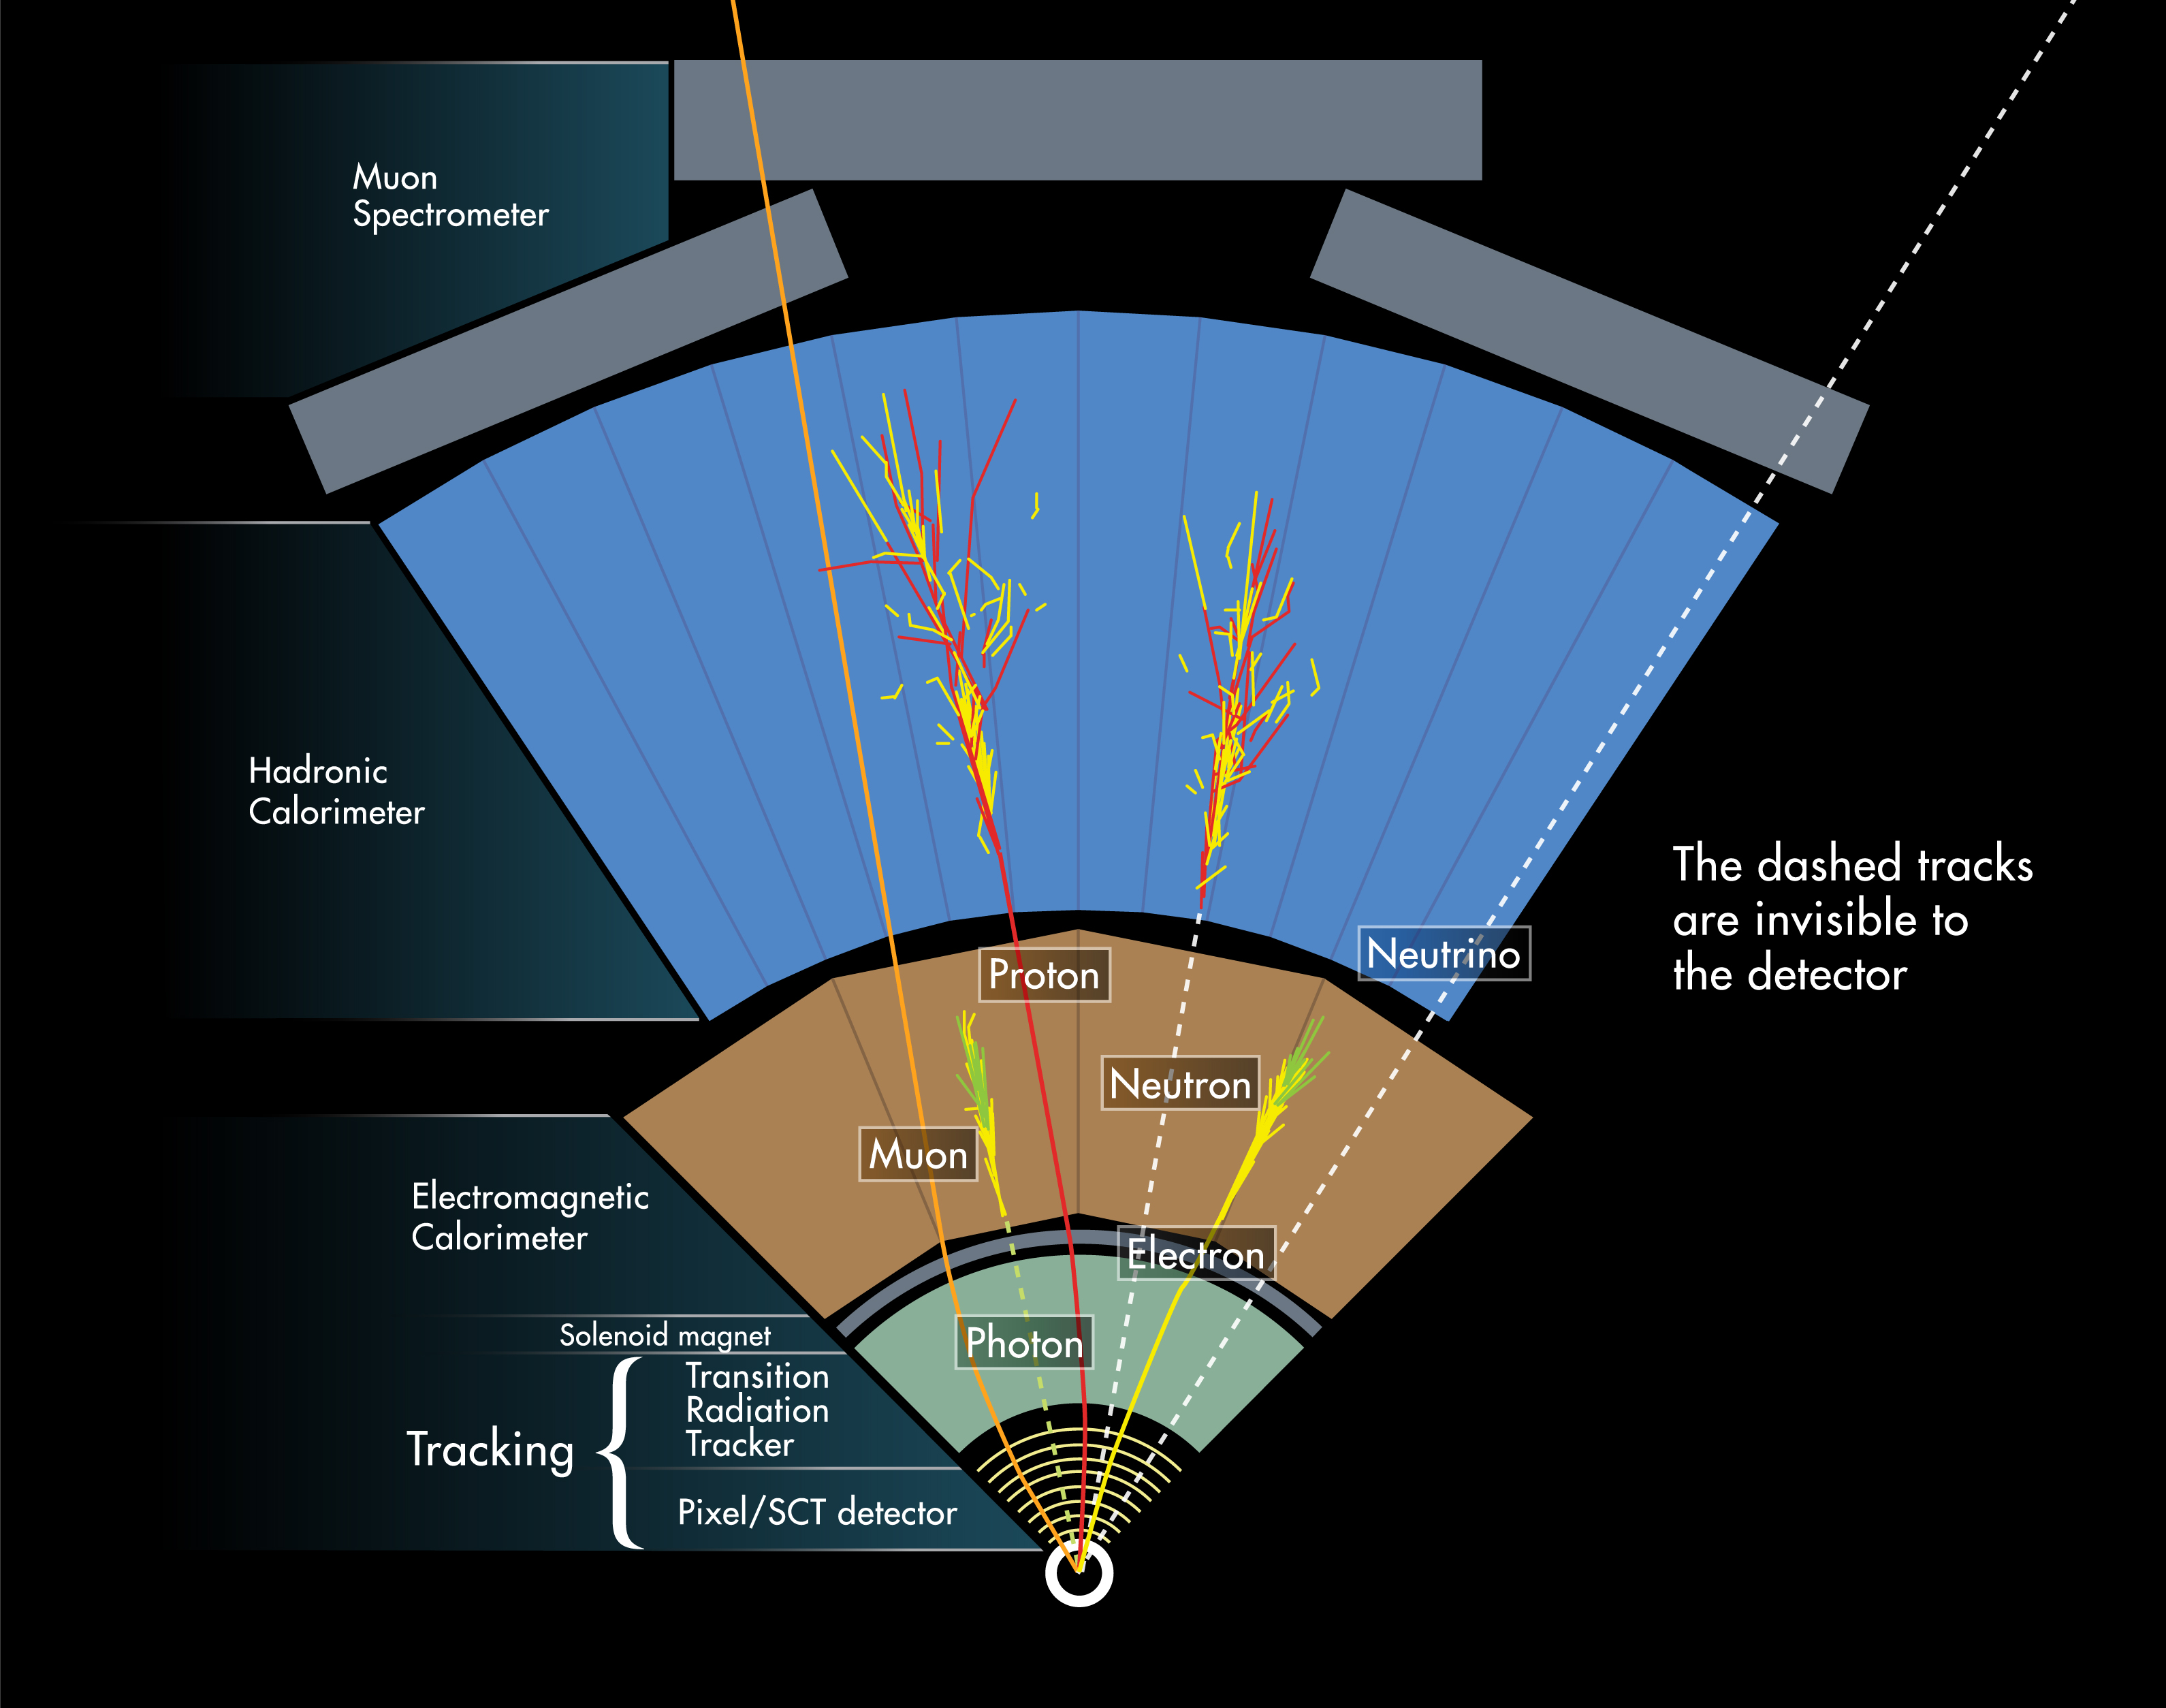
\includegraphics[width=.9\textwidth]{figures/atlas/wedge.jpg}
\caption{A diagram of one wedge of the ATLAS detector
as viewed from looking down the beam line. 
The sub-detector components are shown along with the 
particles that typically come from the collision.
The paths of the particles are shown to indicate how each particle 
might interact with the detector.}
\label{fig:atlas_wedge}
\end{figure}

The geometry of the ATLAS detector is defined using a 
right-handed cylindrical coordinate system with the $x$-axis
pointing inwards towards the center of the LHC ring, the $y$-axis point
up, and the $z$-axis pointing along the beam-line.
The $x-y$ plane, which is perpendicular to the beam-line,
is referred to as the transverse plane and where positions are  
defined using cylindrical coordinates with $r$ being the distance
from the beam-line and $\phi$ being the azimuthal angle.
For describing the direction of the particle with respect 
to the beam-line, a quantity called the pseudo-rapidity, $\eta$, is commonly
used
\begin{equation}
\eta = -\ln \tan (\theta/2) 
\label{eq:pseudorapidity}
\end{equation}
which is a function only of the polar angle, $\theta$, which 
itself is defined
as the direction of the particle with respect to the positive $z$-axis.
Changes in the pseudo-rapidity are 
invariant under Lorentz transformations along
the $z$-axis in the limit that the particle is approximately massless. 
As a result, its distribution is typically flat over
a wide range of pseudo-rapidity. At the LHC, most stable particles 
are produced with energies much larger than their mass, making the 
massless approximation valid.
%The ATLAS detector has nearly uniform $2\pi$ coverage in $\phi$,
%while in $\eta$ the ID is restricted to $|\eta| < 2.5$,
%the MS to $|\eta| < 2.7$, and the calorimeter systems all the way
%to $|\eta| < 4.9$.

The momentum of charged tracks can be measured by measuring how they 
bend in a magnetic field. The deviation of a trajectory
from a straight line path is referred to as the 
sagitta, $s$.\footnote{Technically, the sagitta, $s$, is defined in terms
of an arc as the distance from the center of the arc to the center of its
base. It can related to the radius of the arc, $r$, and the half the length
of the line connecting the two ends of the arc, $l$, by 
$s=r-\sqrt{r^2-l^2}$.} The sagitta is proportional to the magnetic
field strength and inversely proportional to the momentum.
Thus, a straight-line trajectory resembles an infinite-momentum charged
particle (or a neutral particle of any momentum), while
a bent trajectory corresponds to a charged particle with a finite momentum.
As a result, the transverse momentum resolution, $\Delta p_T$, is related to the 
precision on the measurement of the sagitta, $\Delta s$ by
\begin{equation}
\frac{\Delta p_T }{p_T} = \frac{\Delta s}{s}
\label{eq:sagitta}
\end{equation}
This also has the effect that the fraction uncertainty on the momentum
measurement grows linearly as a function of the momentum.


The total momentum of the proton-proton collision in the transverse
plane is nearly zero. Since the detector has full azimuthal coverage 
in the transverse plane, we can test this constraint by measuring
the total momentum from the particles measured in the detector.
The magnitude of a particle's momentum 
in the transverse plane is referred to as the 
transverse momentum, $\pt$.
Thus, we may refer to this constraint as
\begin{equation}
\Bigg| \sum_{i\in\textrm{All Particles}} \vec{p}_{\textrm{T},i} \Bigg| = 0
\end{equation}
where the transverse momentum is added vectorialy and then
the magnitude is taken.
After adding up the $\pt$ of all of the particles to obtain
the total transverse momentum, 
any imbalance with respect to this constraint
is referred to as the
missing transverse energy, $\met$, and is attributed to the 
neutrinos produced in the collision. 
There is no such constraint on the momentum along the $z$-direction
because the momentum fraction of the partons in the collision are not known.
This is the case
even though the momentum along the $z$-direction of the 
protons from which the partons are taken is, in fact, known.
Thus there is no direct way of determining with certainty the 
momentum of the neutrinos in the $z$-direction.



\section{Inner Detector}
\label{sec:atlas_id}

\begin{figure}[ht!]
\centering
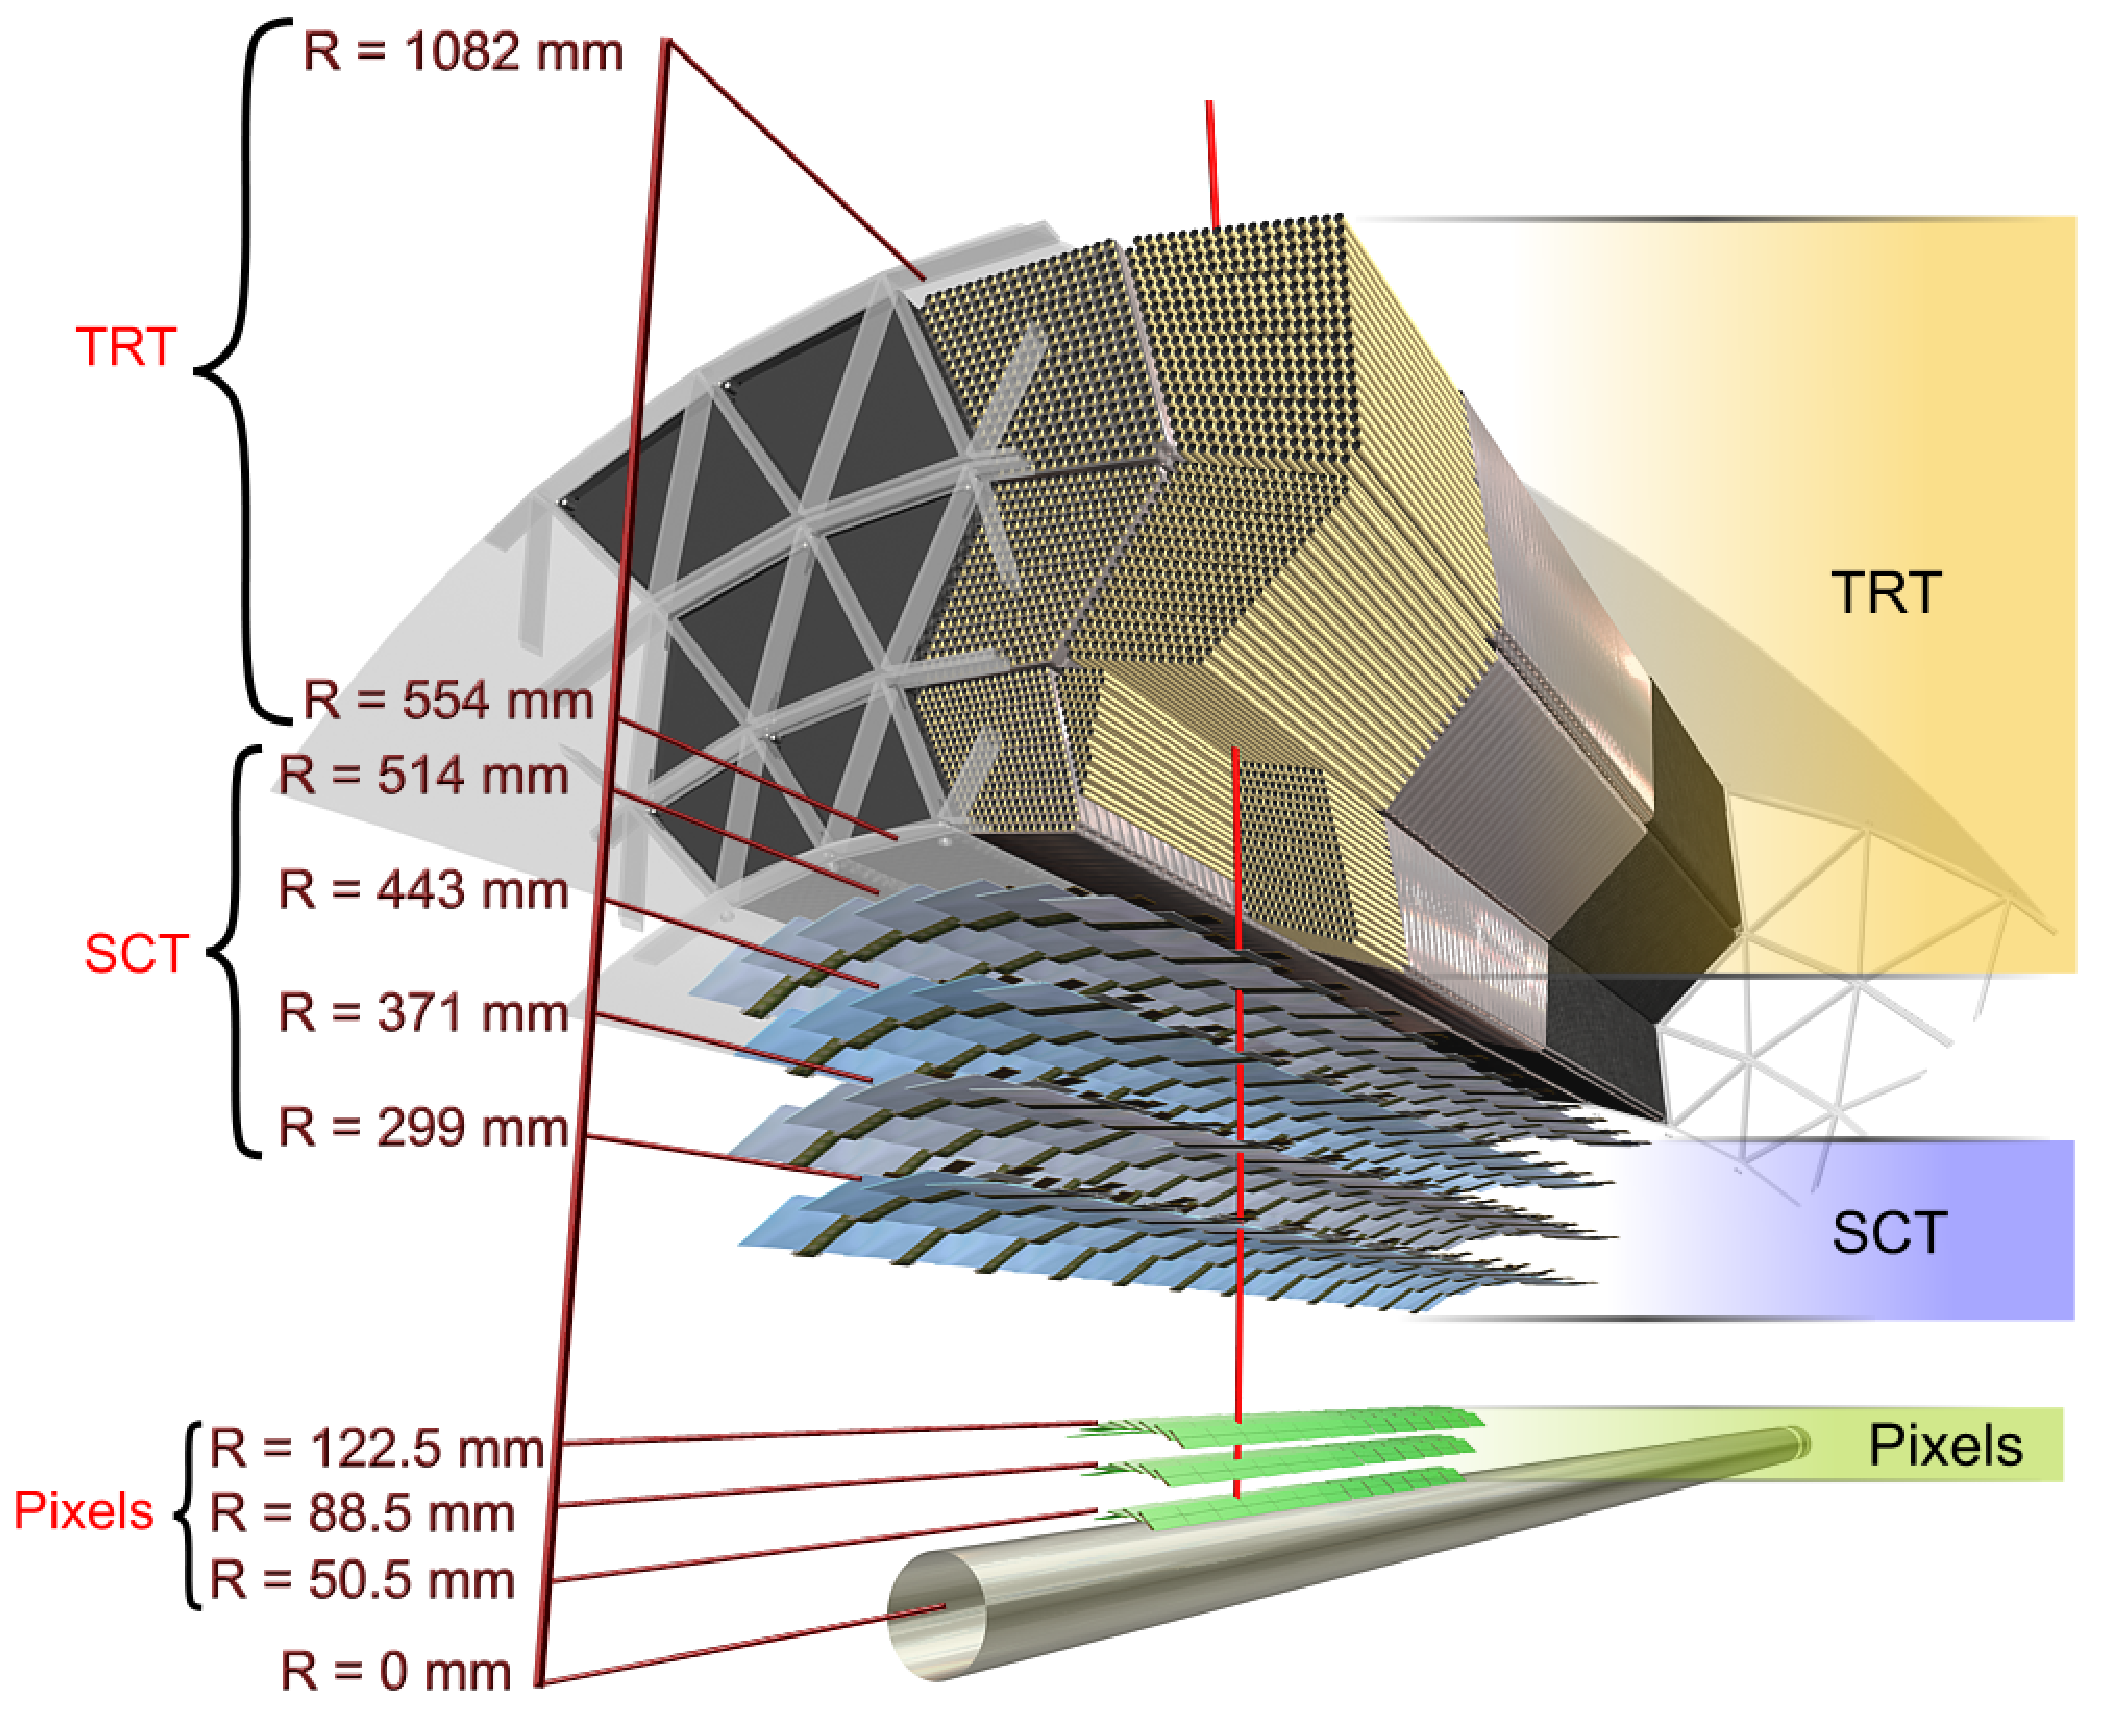
\includegraphics[width=0.7\textwidth]{figures/atlas/id_barrel.eps}
\caption{Diagram of the ATLAS Inner Detector (ID) system showing 
a wedge of the barrel system.  The three detector systems
are clearly labeled. The LHC beam pipe is axial to the system
and is shown at the bottom of the diagram.}
\label{fig:atlas_id_barrel}
\end{figure}

\begin{figure}[ht!]
\centering
\includegraphics[width=0.7\textwidth]{figures/atlas/id_endcap.eps}
\caption{Diagram of the ATLAS Inner Detector (ID) system showing 
a wedge of the endcap system as well as a part of the SCT and Pixel
barrel systems.  The detector systems
are clearly labeled.  The LHC beam pipe is axial to the system
but is not shown. Trajectories of two charged tracks 
with a $\pt=10\GeV$ are shown along $\eta=1.4$ and $\eta=2.2$ are shown 
by the solid bright red lines.}
\label{fig:atlas_id_endcap}
\end{figure}

The inner detector (ID) is the 
detector system that is closest to the beam pipe and thus
first system that the products of the LHC collisions encounter
on their way from the collision point. Its primary role is 
to measure the trajectory and momentum of charged particles
through ionization as they pass through the detector.
It must be capable of measuring these tracks with high precision
in order to obtain precise momentum measurements and also to be able
to accurately extrapolate the tracks back to the collision point
to obtain primary and secondary interaction vertices. In addition,
since the system is so close to the LHC beam line, it
must be able to handle high particle fluxes. This requires that
the ID must have a very high granularity and fast electronics
readouts such that the occupancy of the
detector is small enough to distinguish individual tracks. In addition,
the detector materials and electronics must be sufficiently radiation
hard that they can withstand years of LHC exposure time.
These tough requirements push the limits of available technology and thus
make the ID the most sophisticated detector system in ATLAS.



\begin{figure}[ht!]
\centering
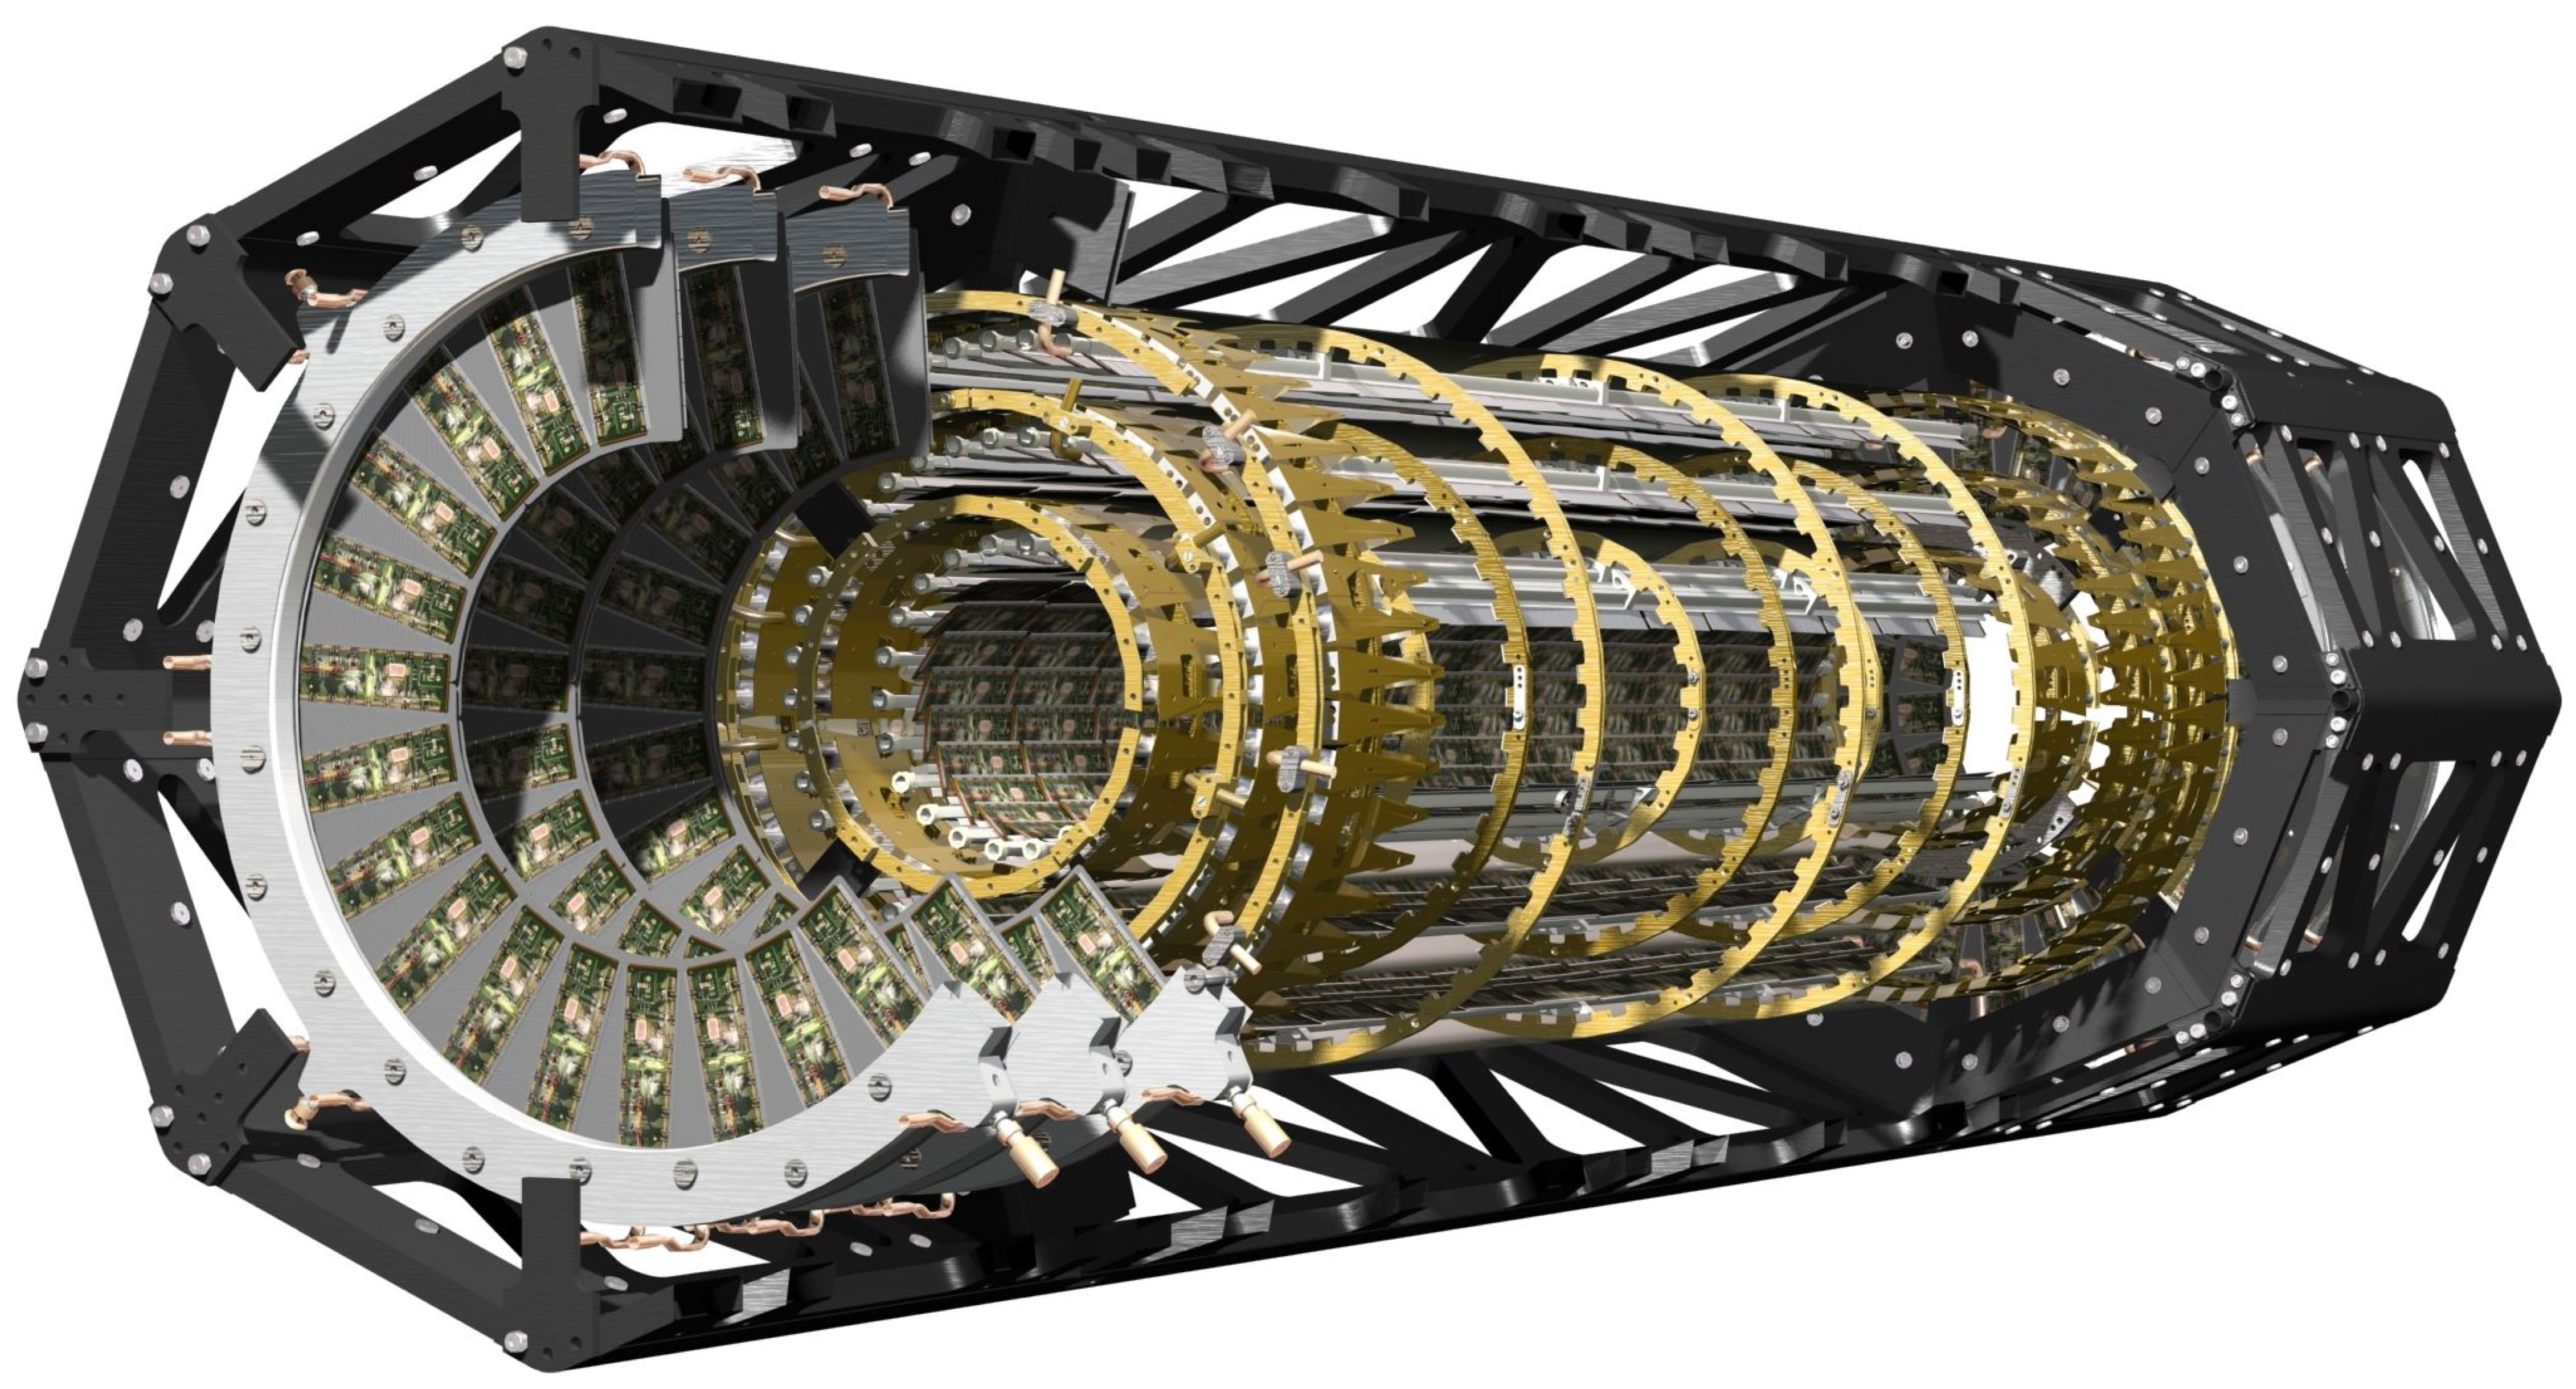
\includegraphics[width=0.7\textwidth]{figures/atlas/pixel.eps}
\caption{A cut-out diagram of the ATLAS pixel detector showing 
the arrangement of the pixel modules (green) in three layers of the barrel
and three layers of one end-cap system. Some of the support structure is
also shown.}
\label{fig:atlas_pixel}
\end{figure}

There are three different detector subsystems within the ID, together
immersed in a uniform 2 Tesla axial magnetic field: the pixel detector,
the silicon microstrip (SCT) detector, and the transition radiation
tracker (TRT). These three detector systems can be seen 
in the barrel in \fig\ref{fig:atlas_id_barrel} and from an alternate
view also showing one of the end-caps in \fig\ref{fig:atlas_id_endcap}. 
The pixel detector
is composed of more than seventeen hundred thin doped silicon sensors with 
dimension $19\times 64~\textrm{mm}^2$. Each sensor has more than forty-six
thousand readout channels,
corresponding to the ``pixels'' which give the detector its name. 
A charged particle passing through an individual pixel produces a signal
which identifies the location of a charged particle. The combination of 
several layers can thus be used to form the trajectory of the particle. %sagitta
Each sensor is attached to a single readout electronic board, which comprises
one module.
The modules are arranged into three cylindrical barrel layers and 
two end-caps each with three disk-shaped layers such that there is uniform
azimuthal coverage. A cut-out diagram of the pixel detector 
structure with modules in place in both the barrel and end-caps is shown 
in \fig\ref{fig:atlas_pixel}. The barrel covers roughly 
$|\eta|<1.7$ and the two end-caps roughly $1.7<|\eta|<2.5$.
Test beam measurements show that the 
spatial resolution of the pixel detector is around $12~\mu\textrm{m}$ in 
the $R-\phi$ plane and is slightly degraded orthogonal to this plane.



The SCT uses almost sixteen thousand thin silicon strip sensors, though not of the 
same type as in the pixel detector. 
A barrel silicon strip sensor has dimension $6.36\times 6.40~\textrm{cm}^2$
with 768 readout strips running along the longer dimension. The barrel
strips are placed in four concentric cylindrical layers, uniformly in azimuth,
with the strips aligned axially, and covering roughly
$|\eta|<1.4$, as can be seen in \fig\ref{fig:atlas_id_barrel}.
In each of the two end-caps the sensors are made to form nine
disks spaced apart along the axial 
direction, covering roughly $1.4 < |\eta|<2.5$, 
seen in \fig\ref{fig:atlas_id_endcap}. The strips are similar
to the barrel except that they are tapered along the strip direction.
The sensors are then oriented such that the taper expands radially outward.
In a test beam, the spatial resolution is found to be about $16~\mu\textrm{m}$
in the $R-\phi$ plane. Due to the length of the strips, the precision is considerably
worse in the axial direction for the barrel and the radial direction for 
the end-caps, with a precision of roughly $580~\mu\textrm{m}$.


The TRT uses a fundamentally different technology 
than the pixel and SCT.
Drift tubes are used of 4~mm in diameter 
which are filled with a Xenon-based gas mixture
and with an anode wire running through the center.
The tubes can be placed in close
proximity such that many measurements, around 36,
can be made on a single charged track. Another important feature
of the TRT is its ability to identify electrons using transition radiation.
This is achieved by surrounding the tubes in polypropylene material to induce
transition radiation from incident particles and taking advantage
of the discrimination power of the Xenon-based gas between 
transition radiation and tracking signals.
For electrons with $\pt>2\GeV$, usually 7 to 10 hits due to transition
radiation will be measured.
The barrel TRT runs from roughly $|\eta|<0.7$ and
is constructed from 144 cm long straws with two straws aligned
axially back-to-back. Over fifty-two thousand straws are interleaved
with polypropylene fibers to form 73 layers of straws surrounding the beam-pipe with
a cylindrical symmetry and uniform coverage in azimuth,
seen in \fig\ref{fig:atlas_id_barrel}.
In each of the two end-caps, two wheels are formed from over seventy-three
thousand straw tubes, 37 cm in length, 
oriented and distributed uniformly in azimuth. 
The inner wheel is formed from twelve layers and the outer wheel from eight
layers with 768 straws in each layer, seen in \fig\ref{fig:atlas_id_endcap}.
The end-caps cover roughly $0.7<|\eta|<2.2$.
An individual straw has a precision of about $170~\mu\textrm{m}$ along
its diameter.




efficiency of electron identification?


large number of readouts?
occupancy??
noise??
sagitta???
explain how the b-field is used?
eta coverage?
materials?
electronics?
more figures?



\section{Calorimeters }
\begin{figure}[ht!]
\centering
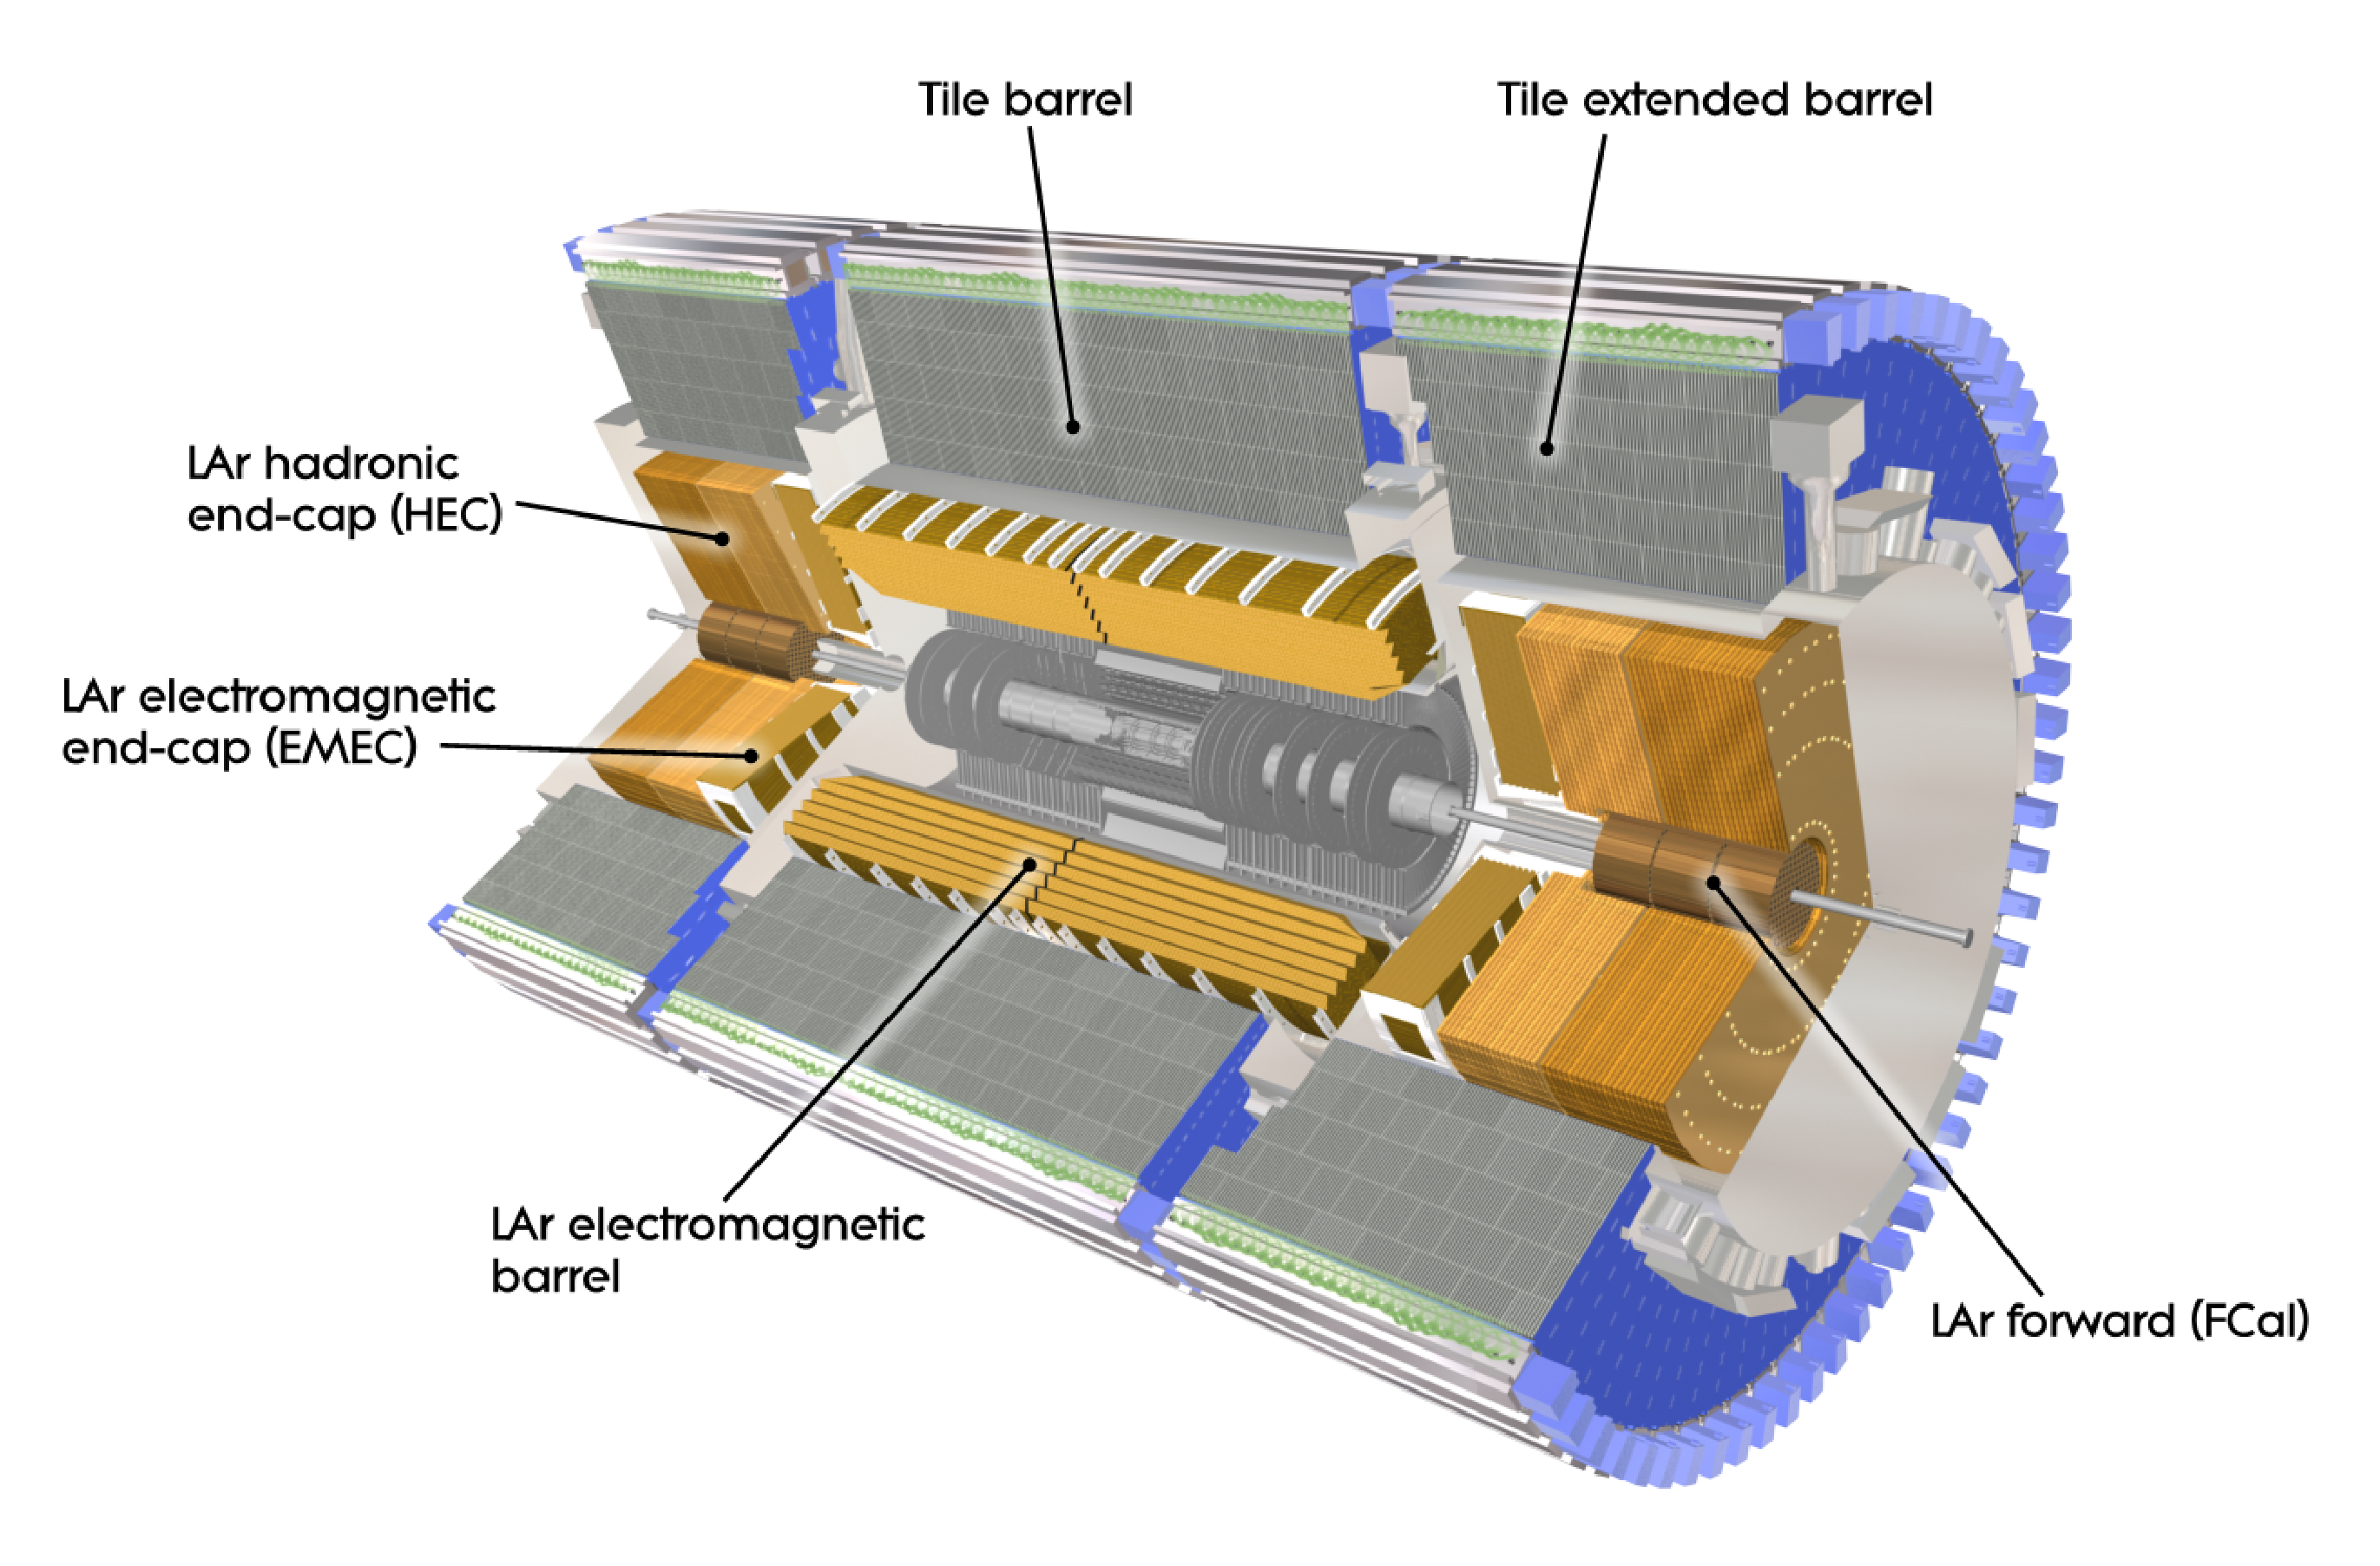
\includegraphics[width=0.9\textwidth]{figures/atlas/calorimeter.eps}
\caption{Diagram of ATLAS calorimeter system with cut-out portion
to allow a view of the nested sub-components.}
\label{fig:atlas_calorimeter}
\end{figure}

The ATLAS calorimeter is designed to measure the energy
deposits of the products of the LHC collisions which pass through
it except for the neutrinos.  A diagram of the 
calorimeter system can be seen in \fig\ref{fig:atlas_calorimeter}.

\begin{figure}[ht]
\centering
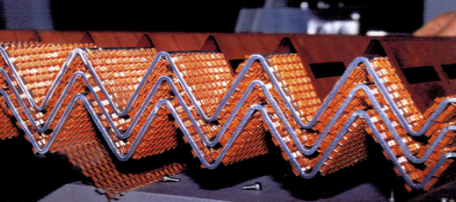
\includegraphics[width=.5\textwidth]{figures/atlas/emcal_accordion.png}
\caption{Photo of three ECAL sampling layers
showing the ``accordion'' structure. In the picture, 
the horizontal directions corresponds to 
the radial direction when the detector is in position, which is
the direction the LHC products would follow.}
\label{fig:atlas_emcal_accordion}
\end{figure}

\begin{figure}[ht]
\centering
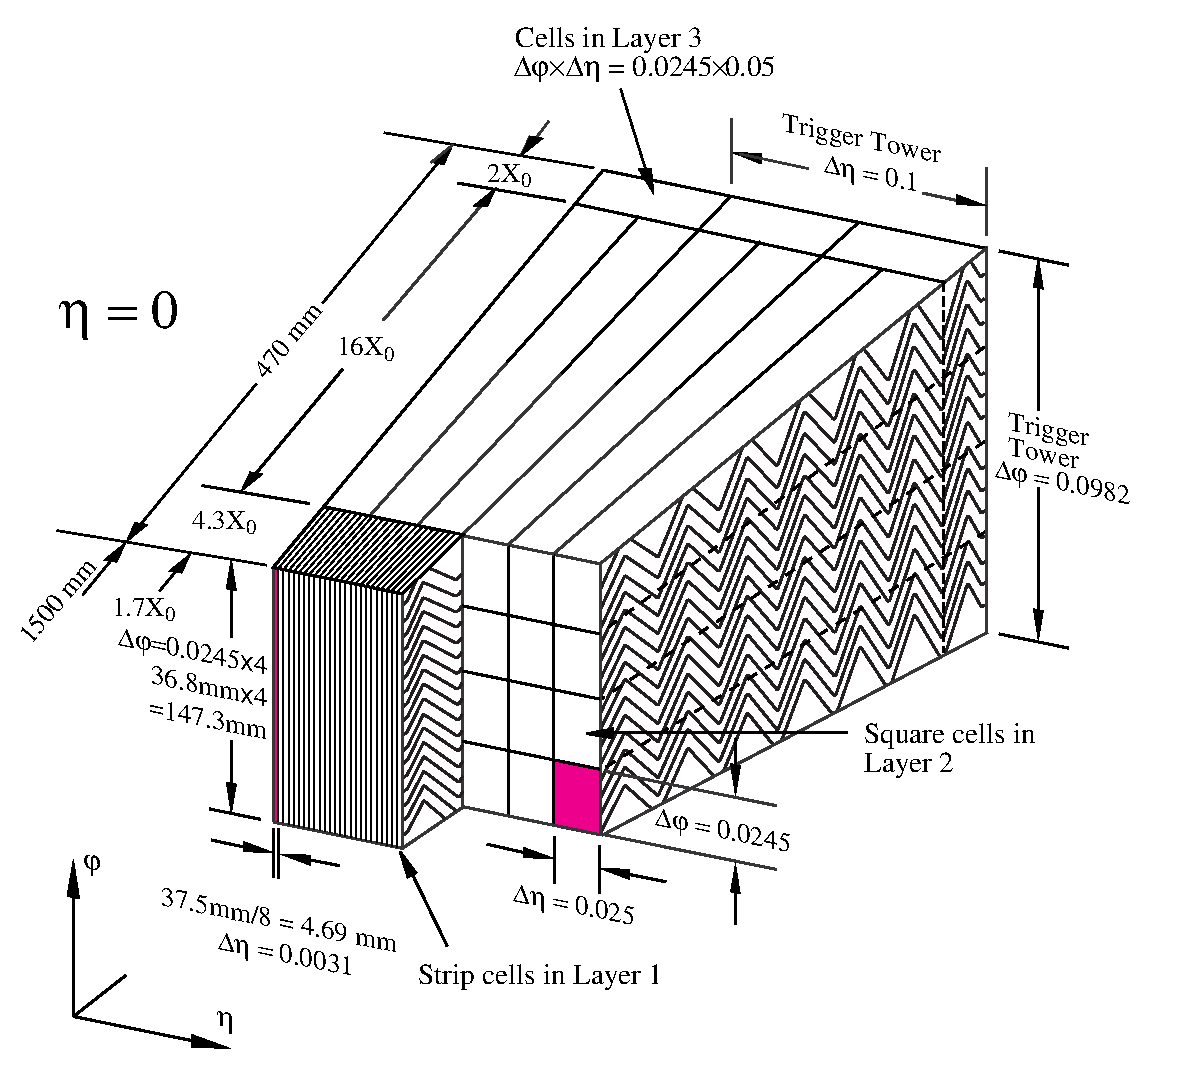
\includegraphics[width=.8\textwidth]{figures/atlas/emcal_barrel_module.eps}
\caption{ A diagram of one ECAL barrel module 
covering $22.5^{\circ}$ in azimuth.}
\label{fig:atlas_emcal_module}
\end{figure}

The calorimeter system is split into three main systems, 
the electromagnetic calorimeter (ECAL), the 
tile hadronic calorimeter (HCAL), the hadronic 
end-cap calorimeter (HEC), 
and the Forward Calorimeter (FCAL).
The ECAL is a sampling calorimeter that uses lead as the sampling
medium and liquid Argon (LAr) as
the active medium from which the charge of the electromagnetic
shower produced by incident particles on the sampling medium
can be collected.  LAr is used as the active medium 
because of its radiation hardness and its linear response.
%as evidenced in \fig\ref{fig:atlas_emcal_response}.
The lead sampling medium alternates with the active LAr medium
using lead plates 1-2~mm thick with an approximately 4~mm 
LAr gap between each sheet and electrodes placed in the middle of
the gaps.
The lead sheets are constructed using a unique ``accordion'' structure,
as seen in \fig\ref{fig:atlas_emcal_accordion}. 
This is to provide a uniform resolution with no gaps
in the azimuthal direction.
The ECAL itself can be split up into a barrel region ranging
from $0<|\eta|<1.3$ and two end-cap regions ranging from 
$1.5 < |\eta| < 3.2$.
The thickness of the barrel region in units of radiation length, \xzero,
ranges from $22~\xzero$ to $30~\xzero$
for $|\eta|<0.8$ and from $24~\xzero$ to $33~\xzero$ for
$0.8 < |\eta| < 1.3$.
The barrel region is divided into individual modules
which together surround the beam-line
in a cylindrical shape.  A diagram of one such module
can be seen in \fig\ref{fig:atlas_emcal_module}.
From this one can see that each module is segmented in $\eta$
and $\phi$, as well as into three layers in depth.
The segmentation is applied to obtain pointing information, 
which aids in the identification and measurement of electromagnetic
objects in conjunction with measurements from the ID.
The very fine segmentation in $\eta$ of the first layer
in depth is important for precision tracking measurements.
The second layer has a larger depth and thus collects most of the energy.
There are two identical end-cap regions, one on each side of the 
collision point. Each end-cap region consists of two wheels: the 
outer wheel from $1.4756 < |\eta| < 2.5$, with a thickness ranging from
$24~\xzero$ to $38~\xzero$, and 
the inner wheel from $2.5 < |\eta| < 3.2$, with a thickness ranging from
$26~\xzero$ to $36~\xzero$.
The regions from $1.5 < |\eta|<2.5$ in the inner and outer wheels both
have three layers, with the first being a finely segmented precision
layer similar to the barrel regions. Outside this region there 
are only two layers with a coarser segmentation.
The ECAL also consists of a pre-sampler detector with a single layer of LAr in 
front of the full barrel ECAL and in front of the end-cap ECAL calorimeters
from $1.5 < |\eta| < 1.8$; this aids in the measurement of the energy deposits
prior to reaching the ECAL and for a better understanding of the energy deposited
in the transition region between the barrel and end-caps.


\begin{figure}[ht]
\centering
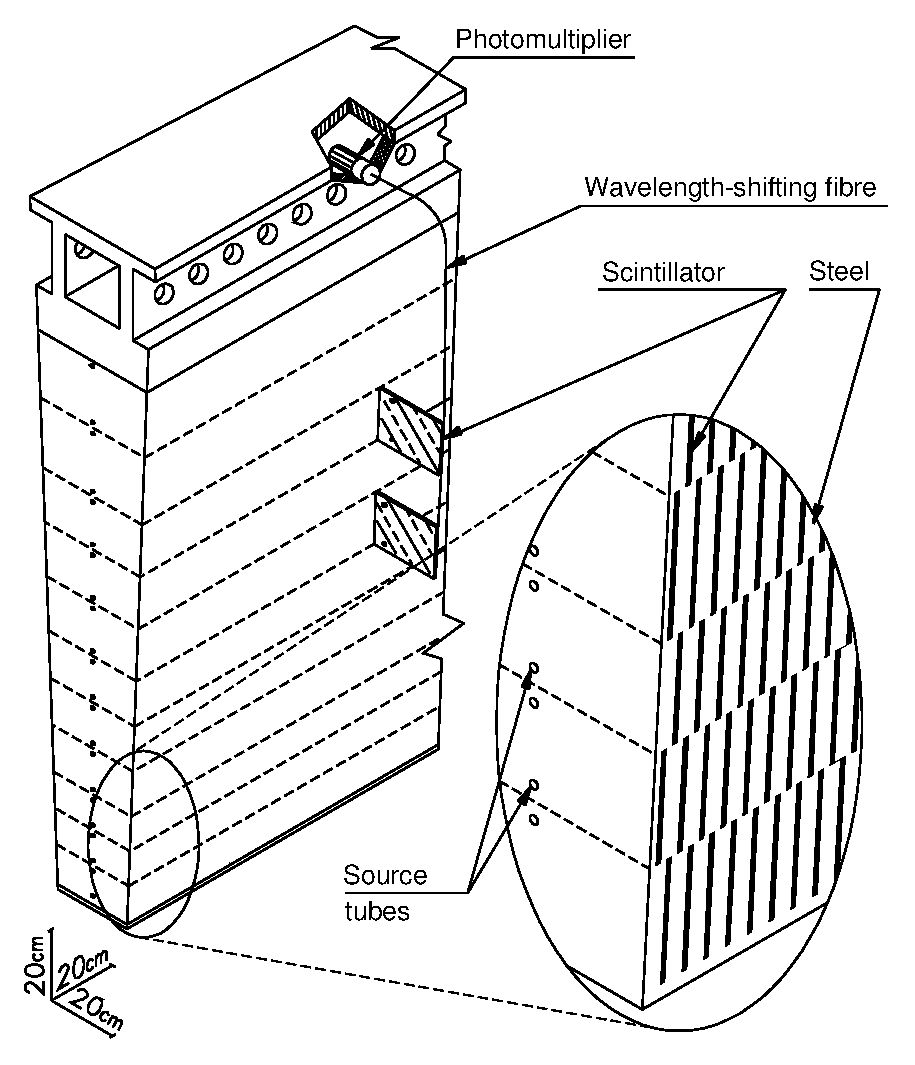
\includegraphics[width=.6\textwidth]{figures/atlas/hcal_module.eps}
\caption{ A diagram of one tile HCAL module 
covering $5.625^{\circ}$ in azimuth. The radial direction when 
positioned in the detector corresponds to the vertical direction in the
image.}
\label{fig:atlas_hcal_module}
\end{figure}


The tile HCAL is a steel sampling calorimeter with scintillating tiles used as the 
active material.
Steel is chosen as the sampling material since it gives a good
depth in interaction lengths, $\lambda$, with a maximum depth
of $7.4~\lambda$, while also having a low cost.
It is split into a central barrel and two extended barrels 
which together cover a 
region from $|\eta|< 1.7$, as can be seen in \fig\ref{fig:atlas_calorimeter}.
As in the ECAL barrel, the tile HCAL is divided into individual modules
that surround the collision point in azimuth; a diagram of one such
module is shown in \fig\ref{fig:atlas_hcal_module}.
The scintillating tiles alternate periodically with the self-supporting
steel body and are oriented radially. 
The scintillation
light is routed through wavelength-shifting fibers and collected
at photo-multiplier tubes placed at the back of the module.
This configuration allows for a near uniform coverage in azimuth.  
In the crack region from $1.2 < |\eta| < 1.6$ between the central barrel 
and extended barrels, special modules are placed to recover and correct
for energy losses in this region.

\begin{figure}[ht] 
\centering
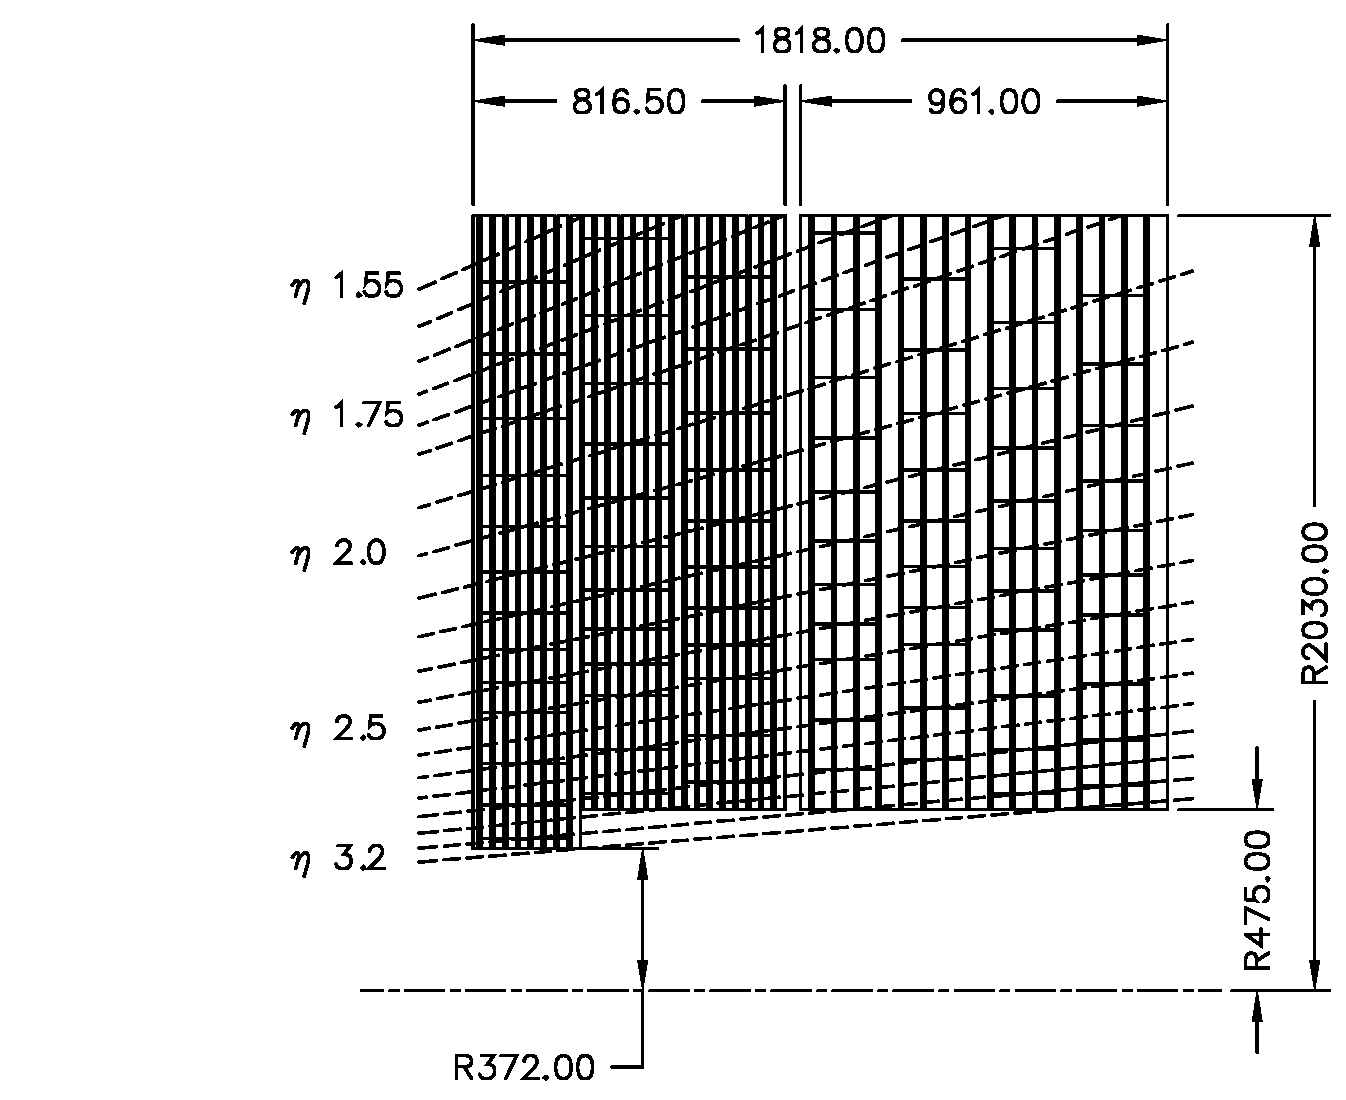
\includegraphics[width=.7\textwidth]{figures/atlas/hec.pdf}
\caption{ A schematic showing one quadrant of the 
HEC system in the $R$-$z$ plane. The dashed lines indicate
the pointing direction achieved by the segmentation of the 
readouts.  Dimensions are in mm.  }
\label{fig:atlas_hec}
\end{figure}


The HEC is designed to measure hadronic energy deposits in the 
end-cap regions from $1.5 < |\eta|< 3.2$. It uses 
copper plates as the sampling material with LAr gaps
for the active material. Two separate wheels are formed from
flat plates of copper alternating with LAr gaps further divided by electrodes for
collecting the ionization charge from the hadronic shower in the LAr.
The rear wheel is more coarse than front wheel;
This can be seen in the schematic of \fig\ref{fig:atlas_hec}.
The electronics readout is segmented such that pointing information
can be obtained, as indicated by the dashed lines.
The maximum radial depth of the HEC is roughly $10~\lambda$.



\begin{figure}[ht] 
\centering
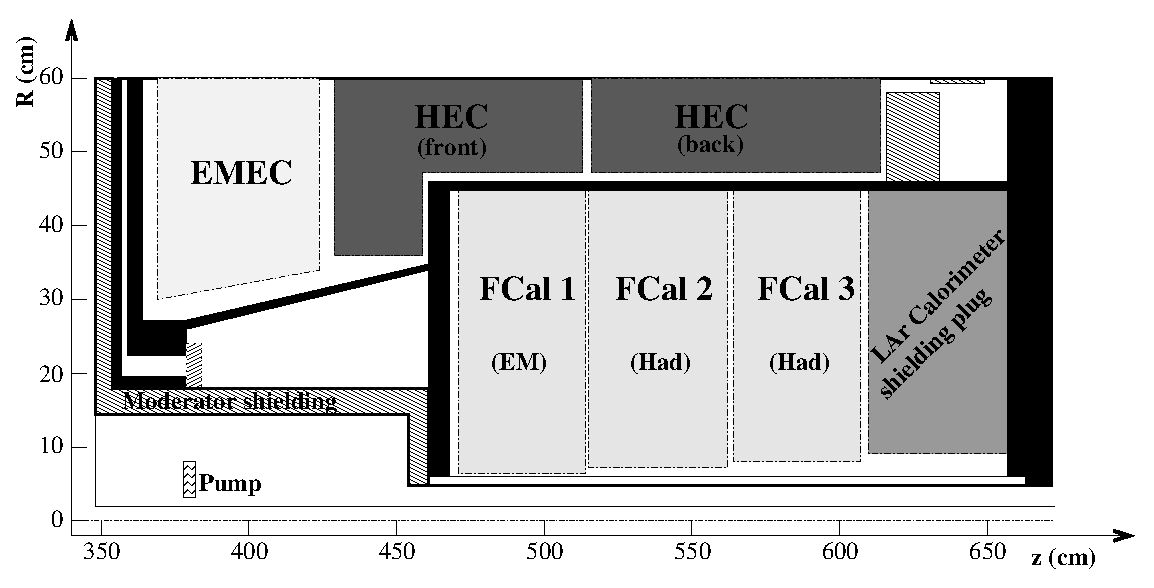
\includegraphics[width=.7\textwidth]{figures/atlas/fcal.eps}
\caption{ A schematic showing the end-cap of the ECAL,
the two HEC modules, and the three FCAL modules, as well
as additional shielding, in one
quadrant of the ATLAS detector as viewed 
in the $R$-$z$ plane.
The $R$-direction is shown with a larger scale than in the $Z$-direction.
}
\label{fig:atlas_fcal}
\end{figure}


The FCAL is in the region of the detector nearest to the beam-line, 
where the radiation flux is highest, covering the range
from $3.1 < |\eta| < 4.9$. It is split into three cylindrical modules,
oriented as in \fig\ref{fig:atlas_fcal}, with the first 
being designed for measuring electromagnetic deposits and the other
two for hadronic deposits.
Each FCAL module is constructed from copper plates with roughly ten thousand
uniformly spaced holes drilled in the direction parallel to the beam-line.
The holes are filled with rods serving as the primary sampling material, 
with a thin LAr gap surrounding the rods serving as the active material.
The first FCAL uses copper rods to optimize for electromagnetic deposits
while the second and third FCAL modules, use tungsten rods
to optimize for hadronic deposits.
The first FCAL has a radiation length of $27.6~\xzero$ and an 
interaction length of $2.66~\lambda$. Meanwhile, the interaction
length of the second and third modules is around $3.6~\lambda$.



Shielding? Resolution and response?




\section{Muon Spectrometer}
%do i want to talk about muon reconstruction?
%definitely mention muon resolution

\begin{figure}[ht]
\centering
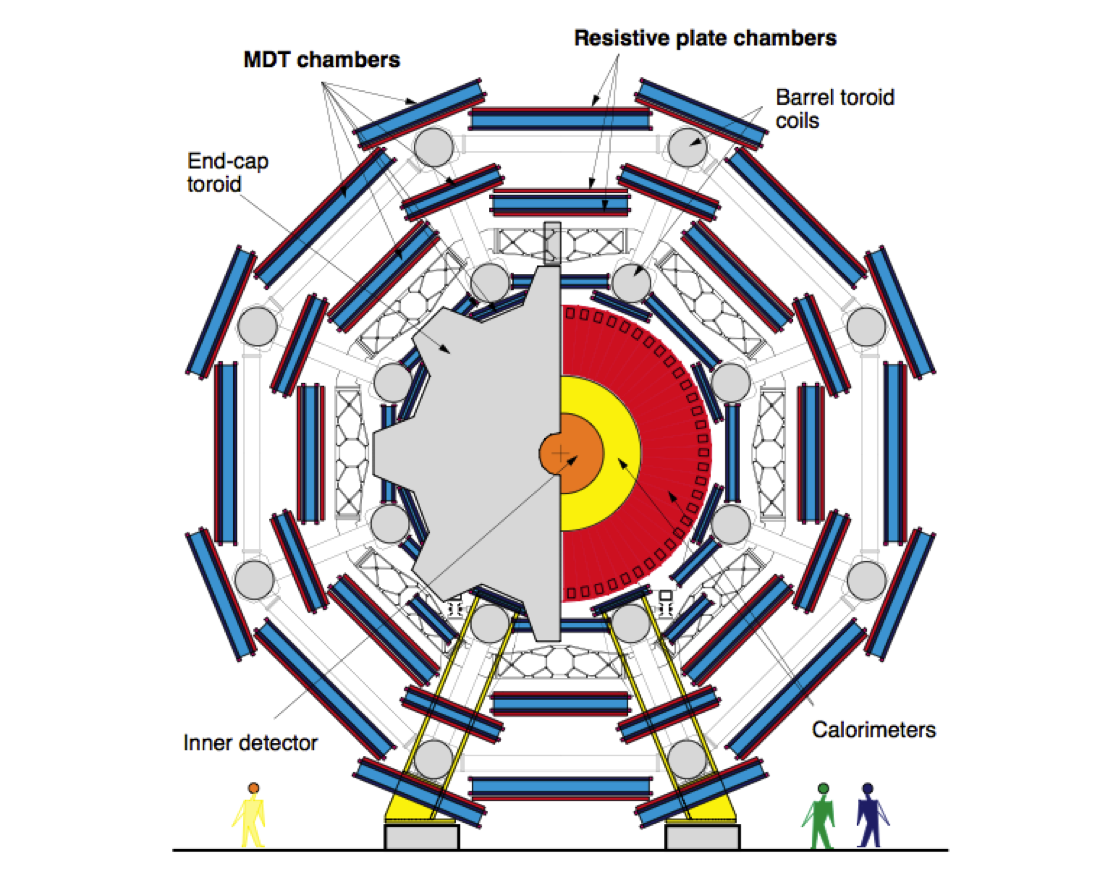
\includegraphics[width=.8\textwidth]{figures/atlas/ms_rphi}
\caption{A cross-section of the MS in the 
transverse ($r-\phi$) plane viewed from one end of the detector. 
The MDT chambers, RPCs, and
barrel and endcap toroids of the MS system are clearly labeled.
The barrel toroid coils extend in to and out of the page while only
half of the endcap toroid is shown to reveal the ID and calorimeter
systems.  The LHC beam pipe runs through the center.}
\label{fig:atlas_ms_rphi}
\end{figure}

\begin{figure}[ht]
\centering
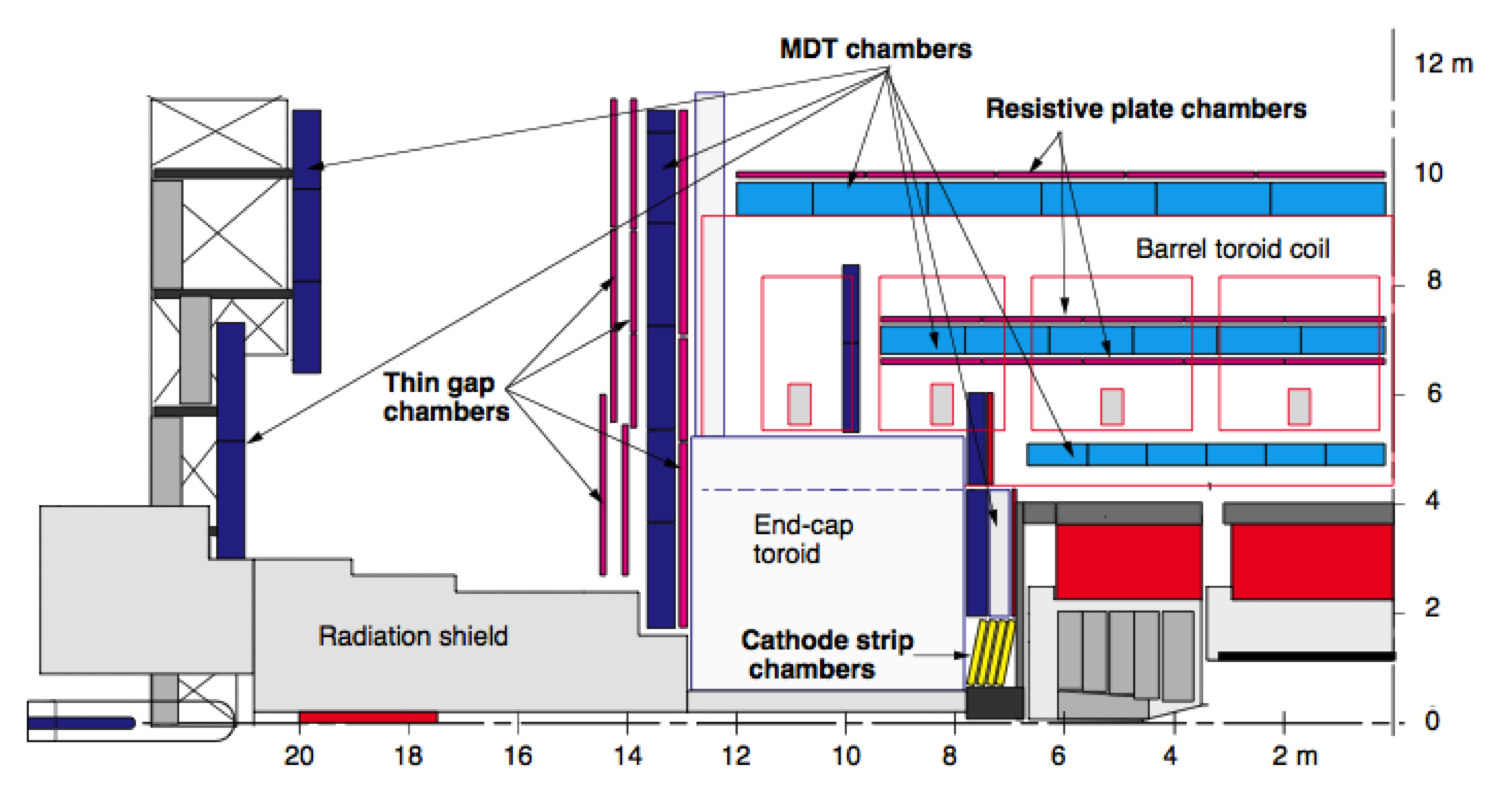
\includegraphics[width=.8\textwidth]{figures/atlas/ms_rz}
\caption{One quadrant of the MS as viewed in the $R-z$ plane. The
MDT chambers, RPCs, TGCs, CSCs are clearly indicated, as are the 
the endcap and barrel toroids. Support structues, shielding and the calorimeter
and ID systems are also drawn. The LHC beam pipe runs from left to right
along the bottom.}
\label{fig:atlas_ms_rz}
\end{figure}

The Muon Spectrometer (MS) is the largest component of the ATLAS
detector, being the component that determines its overall size. 
%The size is determined by the field strength and lever arm...
%maybe try to explain that... look in book that was taken...
It is designed to measure and identify muons as they
pass through the MS and leave the detector.
It surrounds the beam pipe, as well as the ID and calorimeter systems
using a cylindrical geometry with a barrel and two endcaps. 
The MS is comprised of several different technologies:
Muon Drift Tubes (MDT) and Cathode Strip Chambers (CSC) are used as
precision tracking components for measurements of the muon 
trajectory, Resistive Plate Chambers (RPC) and 
Thin Gap Chambers (TGC) are used as fast 
tracking components primarily for triggering, 
and a toroidal magnet system is used for bending the muon trajectory 
in order to extract a momentum measurement.
A diagram of the MS in the transverse plane is shown in 
\fig\ref{fig:atlas_ms_rphi} where the MDT chambers and RPCs of the barrel
are clarly shown along with the barrel and endcap toroids.
Another view of the MS in \fig\ref{fig:atlas_ms_rz} is displayed in
one quadrant along the axial direction which
also shows the barrel and endcap toroids, along with 
the MDT chambers in the barrel and endcap, the RPCs in the
barrel, and the CSCs and TGCs in the endcap.

%The physics requirements are...
\begin{figure}[ht]
\centering
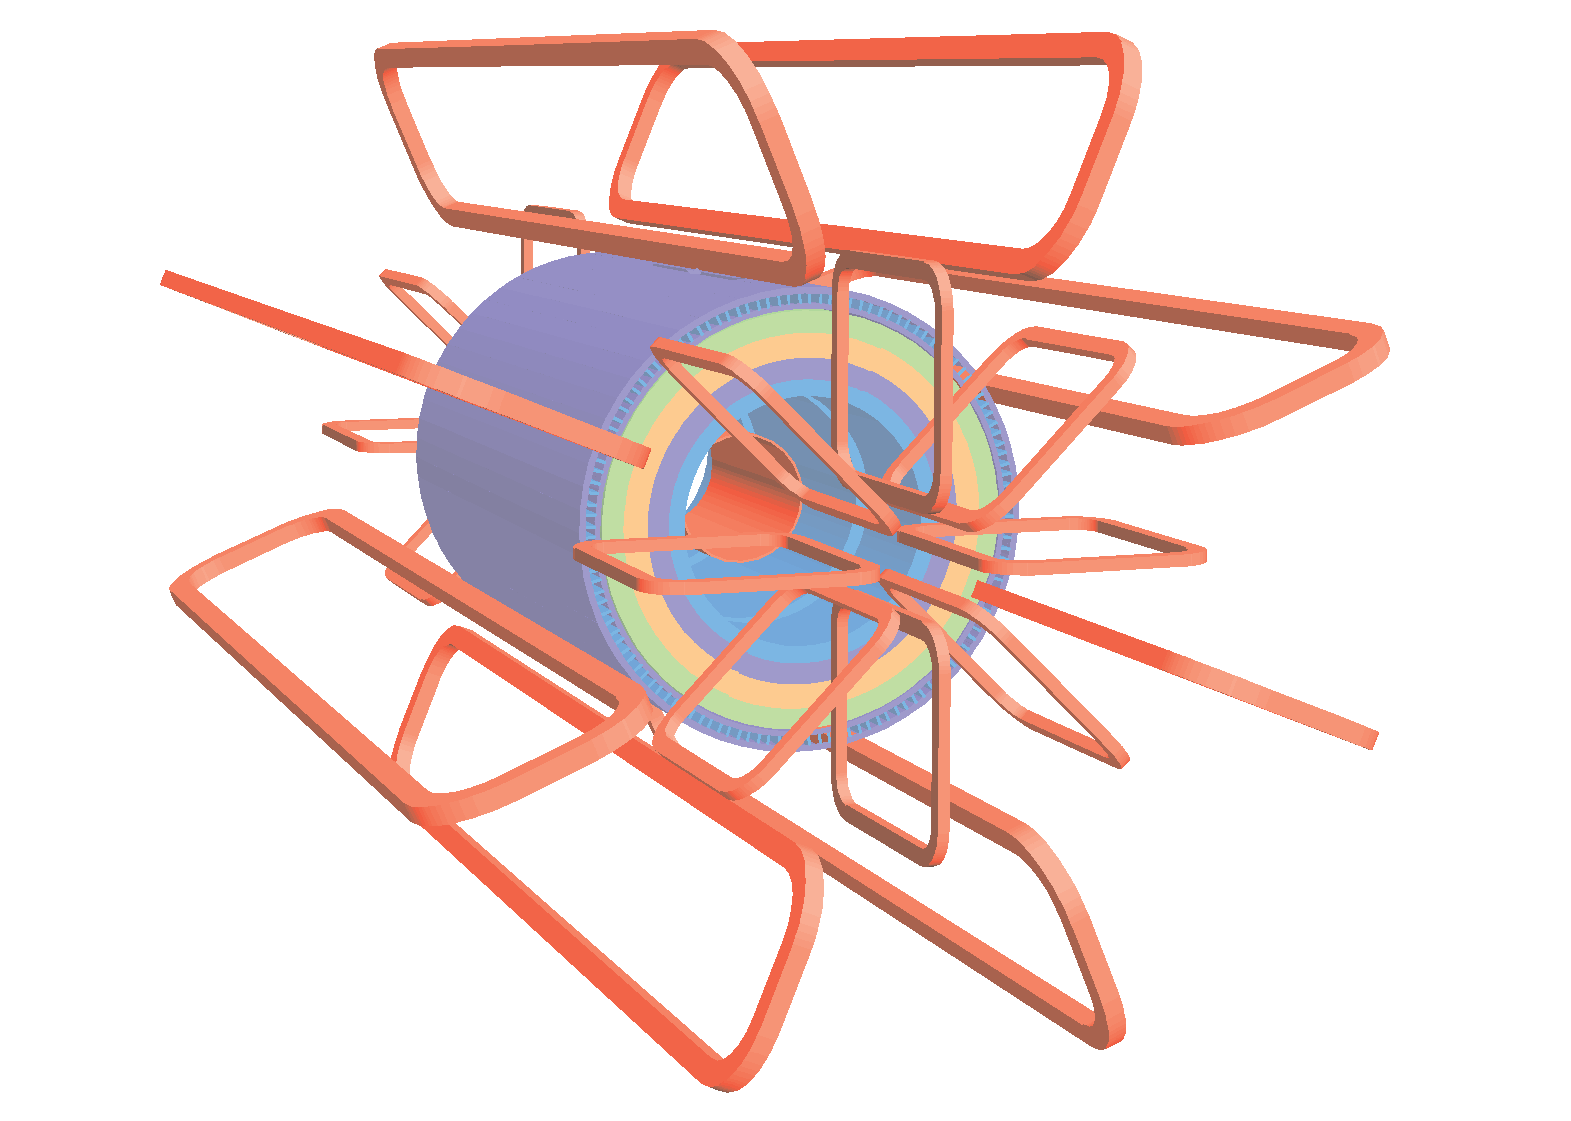
\includegraphics[width=.45\textwidth]{figures/atlas/magnet}
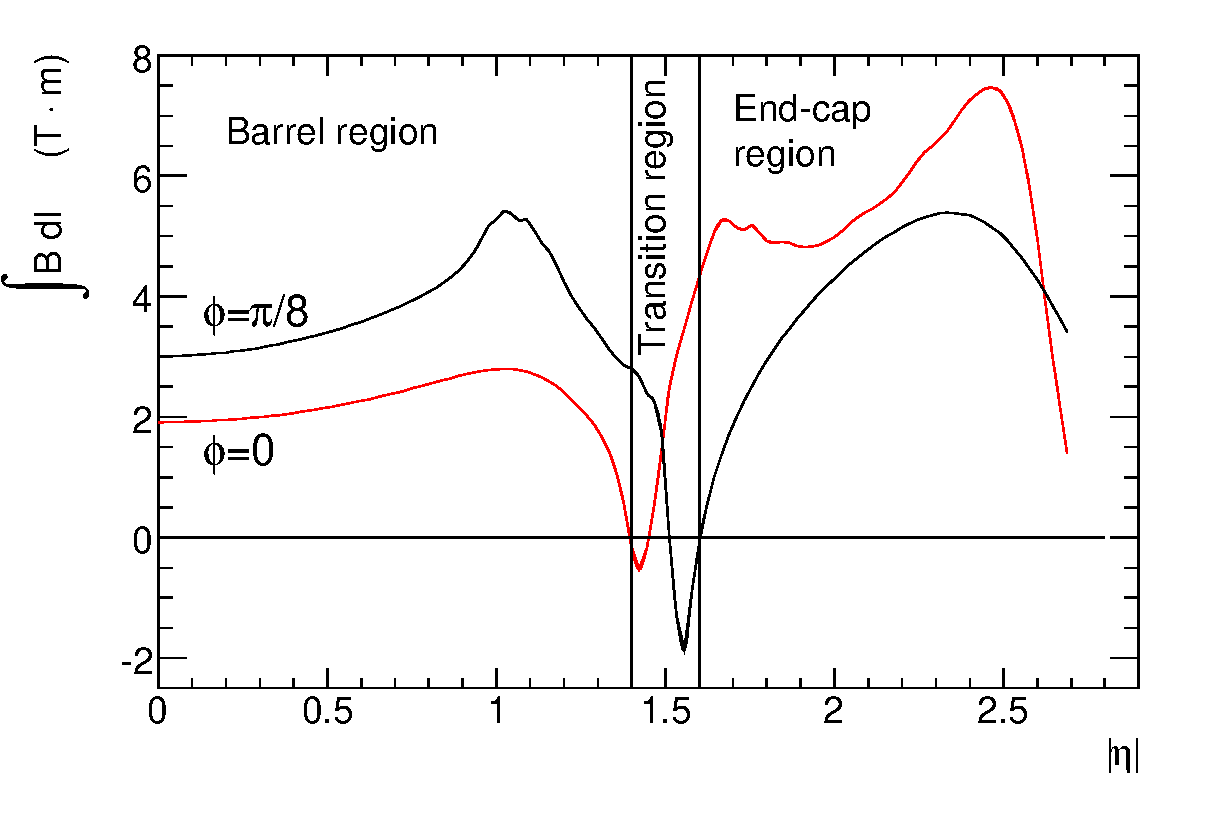
\includegraphics[width=.45\textwidth]{figures/atlas/toroid_magnet_field}
\caption{(\emph{Left}) Diagram of MS toroid magnet geometry (red). The
tile calorimeter is also shown.
(\emph{Right}) Predicted field strength of the MS magnet 
system as a function of $|\eta|$
for $\phi=0$ (red) and $\phi=\pi/8$ (black).}
\label{fig:atlas_toroid_magnet}
\end{figure}


The MS magnet system is composed of several large air-core toroids built
from superconducting coils which produce a magnetic field of 
roughly 0.5 Tesla in the barrel and 1 Tesla in the endcap. 
The geometry of the MS magnet system is shown 
on the left of \fig\ref{fig:atlas_toroid_magnet}. In the barrel, 
eight 25 m long toroidal 
coils insidein stainlees-steel vacuum enclosures are placed uniformly in 
azimuth around the barrel. In the two endcaps, 
each endcap toroid is composed of 
eight square coils (rotated with respect to the barrel toroids)
separated by supporting wedges and then surrounded in a single 
cryostat.
The resulting field is non-uniform as can be seen on the right
of \fig\ref{fig:atlas_toroid_magnet}. 
The field strength in the transverse plane is roughly zero and so is referred
to as the non-bending plane, while the $\eta$ direction is referred to as the
bending plane.
To achieve adequate momentum resolution, the resulting field must be known
precisely.
The field is measured in all directions using sensors placed throughout
the MS and shown to usually agree with predictions within a few milli-Tesla.
The field is especially non-uniform in the region from 
$1.3 < |\eta| < 1.65$, referred to as the transition region, 
where the bending power of the field actually becomes zero
for certain values of $\eta$ and $\phi$.
This results in degraded momentum resolution and poor trigger efficiencies
in this region.


The precision tracking system has stringent requirements
on the precision of the muon trajectory measurement, 
which come from design goals on the resolution of the muon
momentum mesaurement to have a momentum resoution of 
about 10\% at a momentum of 1~\TeV.
Given the magentic field strength in the MS, a muon 
with this momentum is expected to have a sagitta
of about $500\mu$m in the bending plane. 
According to \eqn\eqref{eq:sagitta},
this then translates into a precision requirement of 
no more than $50 \mu$m on the sagitta.
In order to achieve this, MDT chambers are used everywhere 
in the MS from $|\eta|<2.7$, except in the inner layer of the 
endcap from $2<|\eta|<2.7$
where the rates are too high 
and CSCs
are used instead. 
The MDT system is an arrangement of roughly 1000 MDT chambers composed
of aluminum drift tubes roughly 30 mm in diameter and a couple meters in length 
filled with a gas mixture
(Ar/CO2) at a pressure of 3 bar and a high voltage wire (~3000 V)
running through the center. 
It was chosen as the main precision muon tracking system
because of its precision, simplicity and reliability.
When a muon passes through an MDT
it ionizes the gas and electrons are collected at the wire.
The shape (?) of the electron collection pulse on the wire
can be used to determine a radial distance away from the wire
at which the muon passed as in \fig\ref{}. The cylindrical symmetry
of the tube is useful as the resolution is roughly flat, at around
$80\mu$m in the bending plane, as a function
of the angle of incidence of the muon hitting the tube. 
It is not possible, however, to determine the direction
of the muon from just one tube.  For that reason, 
tubes are arranged together in multi-layers of 3-8 tubes such that 
the trajectory
can be reconstructed from matching the patter of hits in multiple layers,
as in \fig\ref{}.
A chamber is built from 2 multilayers separated by a spacer of ... length
giving a precision of roughly $35 \mu$m per chamber.
The long length of the MDTs means that they cannot provide a  useful measurement
in the non-bending plane.
Chambers are arranged in three concentric shells in the barrel 
at $r = $5 m, 7.5 m, and 10 m and in several rings in the endcap
at $|z| = $7.4 m, 10.8 m, 14 m, and 21.5 m as in \fig\ref{}.
In each shell or ring
the chambers are made to overlap in order to avoid gaps in azimuth.
Still, there are gaps, in particular around $|\eta|=0$ due to a hole for services
and due to the feet holding up the detector, seen in \fig\ref{fig:atlas_ms_rphi}.
An optical alignment system is used to monitor the MDT chambers %alignment between chambers?
for deformations and the tension of the wires can be adjusted
to adjust for sag where needed. %technically only in barrel.
Despite having very good precision, the maximum drift time
can be as high as 700 ns, which is far too slow for LHC bunch identification.


The CSC are used in the region of the MS closest to the interaction
point where the crossing rate of tracks 
is greater than $150$ Hz/cm$^2$, 
too high for succesful operation of the MDT chambers.
The CSCs can handle up to 1000 Hz/cm$^2$
while maintaining adequate  precision in the bending plane.
A CSC is a multiwire proportional chamber
composed of layers of cathode strips sandwhiching 
a set of anode wires and filled with a non-circulating gas (Ar/CO2).
The two sets of cathode strips in a layer are separated by 5mm
with the anode wires running directly between the two sets.
In each layer the the two sets of cathode strips are segmented in
orthogonal directions in order to give 
A signal is induced on the cathode strips due to an avalanche
of electrons from the ionizing muon collecting on the anode wire.
The two sets of cathode strips are segmented in orthogonal directions
providing measurements in both the bending and non-bending planes. 
A CSC is composed of four layers, each giving separate $\eta$ and
$\phi$ measurements.
The resolution in the bending plane is roughly 60 microns
while the coarser segmentation in the non-bending plane 
results in a  resoulution of  roughly 5 mm.
Two rings are formed from the chambers such that the anode wires
point radially and that there are no gaps in $\phi$, as
can be seen in \fig\ref{}. The rings are positioned
at roughly $|z|=7.5$ m. The rectangular symmetry 
results in a degradation of the resolution based on the angle of incidence.
This is resolved by titling the chambers slightly toward the interaction point.
Of use in the high occupancy environment, 
if multiple tracks are present in a CSC in a given event, 
the signal pulse height can be used to match the tracks.
The small separation between cathode strips results in a layer
results in a short electron drift time allowing for a good
timing resolution of about 7 ns per layer.

optical alignment?

show resolution plot (something about this in 2.2.1)

The fast tracking system in the MS is designed to be able
to identify muons coming from individual bunch crossings of the LHC
and to discriminate them based on their position and \pt in the region
$|\eta|<2.4$. This information
is then used to trigger on high \pt~muons, as 
described in \sec\ref{sec:atlas_trigger}.
The individual bunch crossings of the LHC are designed to 
be separated by only 25 ns, as described in \sec\ref{sec:lhc}.
Thus, the system must be able to resolve individual tracks 
with a time resolution of this size (what exactly is the design req?).
To distinguish high \pt~muons from straight-track neutral particles 
or highly curved-track low-momentum charged particles, the 
system must be able to measure the sagitta of the 
trajectory in the toroidal magnetic field, though not 
with the same precision as in the precision tracking system.
Furthermore, to distinguish individual tracks, position measurements
must be performed in both the bending and non-bending planes.
The measurement in the non-bending plane is also used to complement
the measurements of the bending plane from the MDT chambers.
In order to achieves this, RPCs are used in the barrel region
from $|\eta|<1.05$ and TGCs in the endcap from $1.05 < |\eta|<2.4$.
The layour of the fast tracking system can be seen in the diagram
in \fig\ref{fig:atlas_muon_fast_tracking}. %use figure 6.27
The RPCs are parallel electrode-plate detectors which use no wires.
A single RPC layer consists of 
resistive plates aligned in parallel and separated by 2 mm 
with a gas mixture (primarily $\textrm{C}_2\textrm{H}_2\textrm{F}_4$)
in the gap. An electric field of 4.9 kV/mm is applied between 
the plates which results in electron avalanches to form in the gas
along track toward the anode plate.
This gives a signal pulse time resolution of about 5 ns.
The pitch of the individual plates is 23 mm in $\eta$ and 35 mm in $\phi$
A single RPC consists of two layers.  Three concentric shells 
are formed from the RPCs around the beam line at about $r = $ 6.5, 7.5, and 10 m
as in \fig\ref{fig:atlas_muon_fast_tracking}.
The separation between the inner and outer layers 
allows for a discrimination of muons with $9 < \pt < 35~\GeV$
while the separation between the inner and middle layers allows for 
discrimination of low-\pt~muons with $6 < \pt < 9~\GeV$.
Space resolution...maybe put sqrt(12) formula? look up to be sure.


The TGCs are multi-wire proporational chambers, similar to the CSCs.
In a single TGC layer,the cathodes are separated by 2.8 mm and the wire-to-wire pitch
is 1.8 mm.  A high voltage of 2900 V is applied to the anode wires
resulting in a quasi-saturated electron avalanche in the gas 
mixture (CO2/n-pentane) due to incident tracks.
The small wire-to-wire pitch and high voltage result in a good 
timing resolution for the signal pulse. The resulting
signal pulse resolution is dependent on the angle-of-incidence
of the incoming track, but still results in a signal width
within 25 ns for about 99\% of tracks.
TGC chambers are built from either two are three layers. 
The TGC chambers are then arranged in rings such that they overlap
in azimuth to eliminate gaps.
The TGC rings are arranged as in 
as in \fig\ref{fig:atlas_muon_fast_tracking}
with a ring of two-layer TGCs placed in front of the endcap MDT inner
layer at about $|z|=7$ m, 
a ring of three-layer TGCs placed in front of the endcap MDT
middle layer at around $|z|=13 $m, and two rings of 
two-layer TGCs placed just behind
the endcap MDT middle layer at around $|z|=14$ m.
pt resolution and performance?



\section{Trigger}
\label{sec:atlas_trigger}

\section{LUCID?}
